\documentclass[a4paper]{article}
\usepackage[english, mongolian]{babel}
\usepackage[utf8x]{inputenc}
\usepackage{graphicx}
\usepackage{listings, paralist}
\usepackage{xcolor}
\usepackage{float}
\usepackage{url}
\usepackage{amsmath}
\usepackage{amssymb}
\usepackage{multirow}
\usepackage{multicol}
\usepackage{titlesec}
\usepackage{geometry}
\usepackage{indentfirst}
\usepackage{booktabs}
\usepackage{adjustbox}
\usepackage{dblfloatfix}
\usepackage{mdframed}
\usepackage[tc]{titlepic}
\usepackage{blkarray}
\usepackage{pythonhighlight}
\usepackage[
    backend=bibtex,
    style=ieee
]{biblatex}
\addbibresource{citation.bib}

\tolerance=1
\emergencystretch=\maxdimen
\hyphenpenalty=10000
\hbadness=10000

\geometry{
  left=2cm, % Adjust the left margin
  right=2cm, % Adjust the right margin
  top=2cm, % Adjust the top margin
  bottom=2cm, % Adjust the bottom margin
}
\setlength{\columnsep}{0.8cm}
\setlength{\columnwidth}{\dimexpr(\linewidth-\columnsep)/2}
\fontsize{10pt}{12pt}\selectfont
\titleformat{\section}[block]{\bfseries}{\thesection.}{1em}{} 
\titleformat{\subsection}[block]{\hspace{2em}}{\thesubsection}{1em}{}

\title{Хэв танилтын үндэс Лаборатори 2-2 тайлан}
\author{Эрдэнэ Тэмүүжин - 20B1NUM1970}
\date{\today}
\begin{document}
% ----------------------------------------------------------------
\begin{titlepage}
\begin{center}
 {\huge\bfseries Хэв танилтын үндэс \\ Лаборатори 2-2 тайлан\\}
 % ----------------------------------------------------------------
 \vspace{1.5cm}
 {\Large\bfseries Эрдэнэ Тэмүүжин}\\[5pt]
 20b1num1970@stud.num.edu.mn\\[14pt]
  % ----------------------------------------------------------------
 \vfill
 % ----------------------------------------------------------------

\includegraphics[width=0.19\textwidth]{logo_web.jpg}\\[5pt]
\Large
ХШУИС Хэрэглээний Математикийн тэнхим\\
Монгол Улсын Их Сургууль\\
\vfill
{2023 оны 10-р сарын 12}
\end{center}
\end{titlepage}
% ----------------------------------------------------------------
\maketitle
\begin{center}
    \vspace{-1em}
    МУИС-ХШУИС Хэрэглээний Математикийн тэнхим \\
\end{center}
\section*{\centerline{Удиртгал}}
Өмнөх лабораторийн ажилд дижитал зургийн пиксел нэг бүрийн утгад хандаж зурагт босго тогтоох эсвэл зургийн ялгарлыг нэмэгдүүлж байсан бол энэ лабораторийн ажилд зургийн тодорхой орчин дахь пикселийн утгуудад хандана.
\section{Histogram Processing}
Дижитал зургийн гистограм нь уг зургийн пикселийн эрчмийн үзэгдэх магадлалыг буцаадаг функц юм \cite{gonzalez2009digital}. 
\begin{equation}
p_r(r_k) = \frac{n_k}{MN}, \quad k = 0, 1, ..., L - 1
\end{equation}
Энд $n_k$ нь $r_k$ эрчимтэй пикселийн тоо, харин $MN$ нь зургийн нийт пикселийн тоо. $L$ нь зургийн авч болох боломжит эрчмийн тоо. Эндээс зургийн эрчмийн хуримтлагдсан тархалтын функцийг тооцно \cite{gonzalez2009digital}.
\begin{equation}
s_k = \frac{L-1}{MN} \sum_{j=0}^{k} n_j, \quad k = 0, 1, ..., L-1
\end{equation}
Тэгэхээр оролтын зургийн пикселийн эрчмийг хуримтлагдсан тархалтын утга бүрд нь харгалзуулснаар гаралтын зураг үүсэх юм.
\begin{figure}[H]
  \centering
  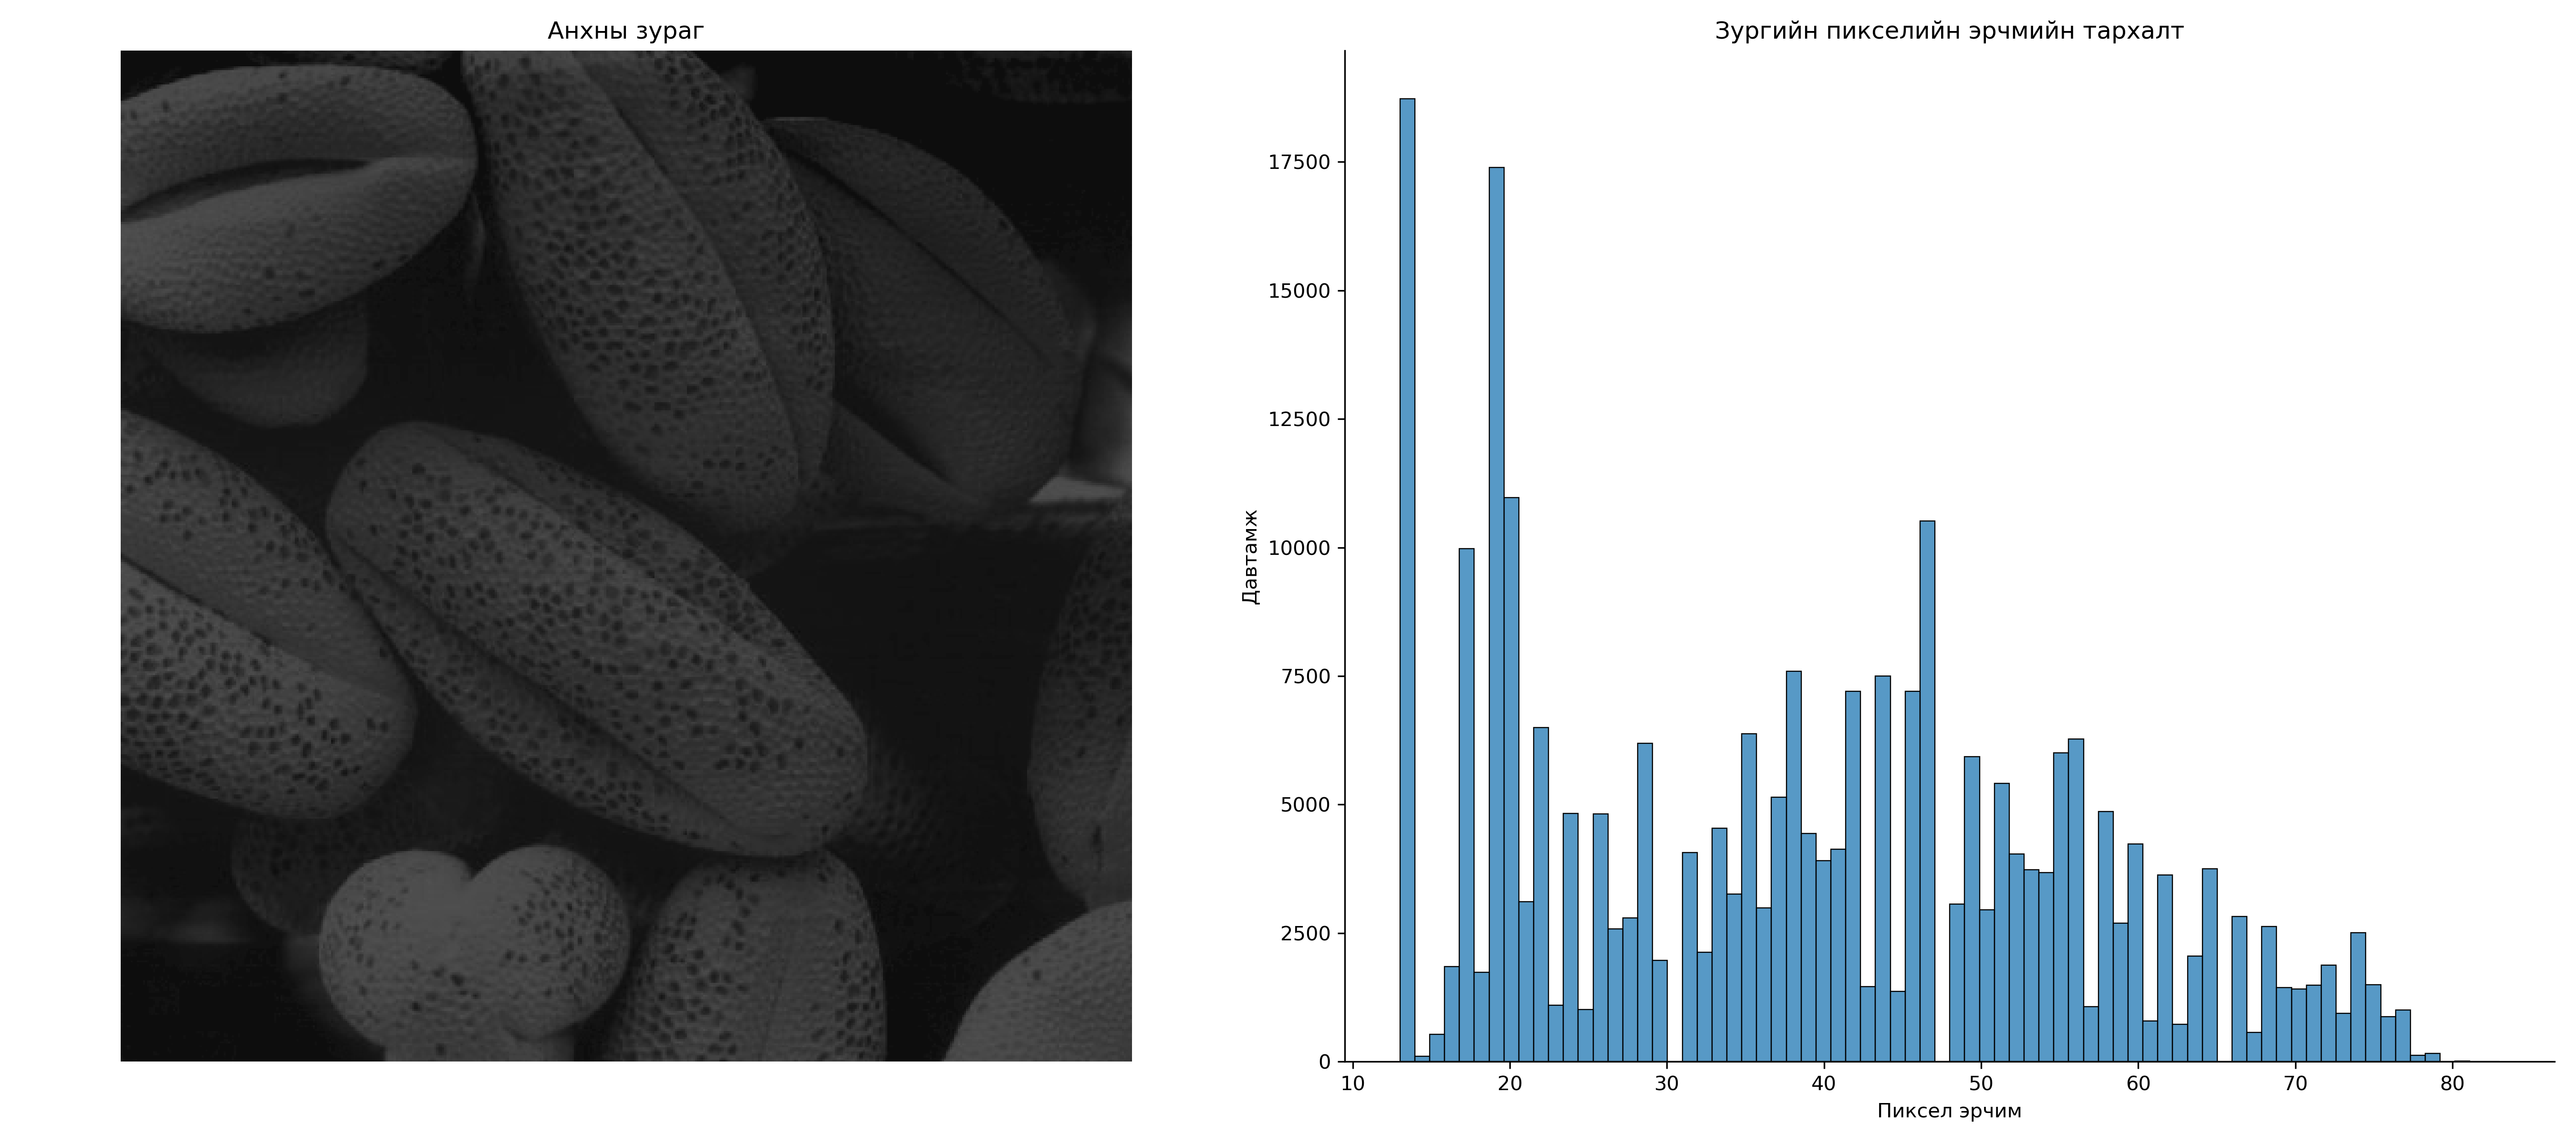
\includegraphics[scale = 0.30]{global_hist_eq_task_1.png}
  \caption[Intensity 1]{Оролтын зураг ба эрчмийн тархалт}
\end{figure}
\begin{python}
def imhist(img):
    row, col = img.shape
    h = [0] * 256

    for i in range(row):
        for j in range(col):
            h[img[i, j]] += 1
    
    return np.array(h)/(row*col)

def cumsum(h):
    return [sum(h[:i+1]) for i in range(len(h))]

def hist_eq(img):
    h = imhist(img)
    cdf = np.array(cumsum(h)) 
    sk = np.uint8(255 * cdf)
    s1, s2 = img.shape
    Y = np.zeros_like(img)
    
    for i in range(s1):
        for j in range(s2):
            Y[i, j] = sk[img[i, j]]
            
    H = imhist(Y)
    return Y, h, H, sk
\end{python}
\textit{imhist} функц болон \textit{cumsum} функцүүдэд пикселийн эрчмийн гистограм болон хуримтлагдсан тархалтыг гараар тооцож байгаа. Үүний дараагаар \textit{hist\_eq} функц ашиглан гаралтын зургийг тооцож байна.
\begin{python}
for i in range(s1):
        for j in range(s2):
            Y[i, j] = sk[img[i, j]]
\end{python}
\begin{figure}[H]
  \centering
  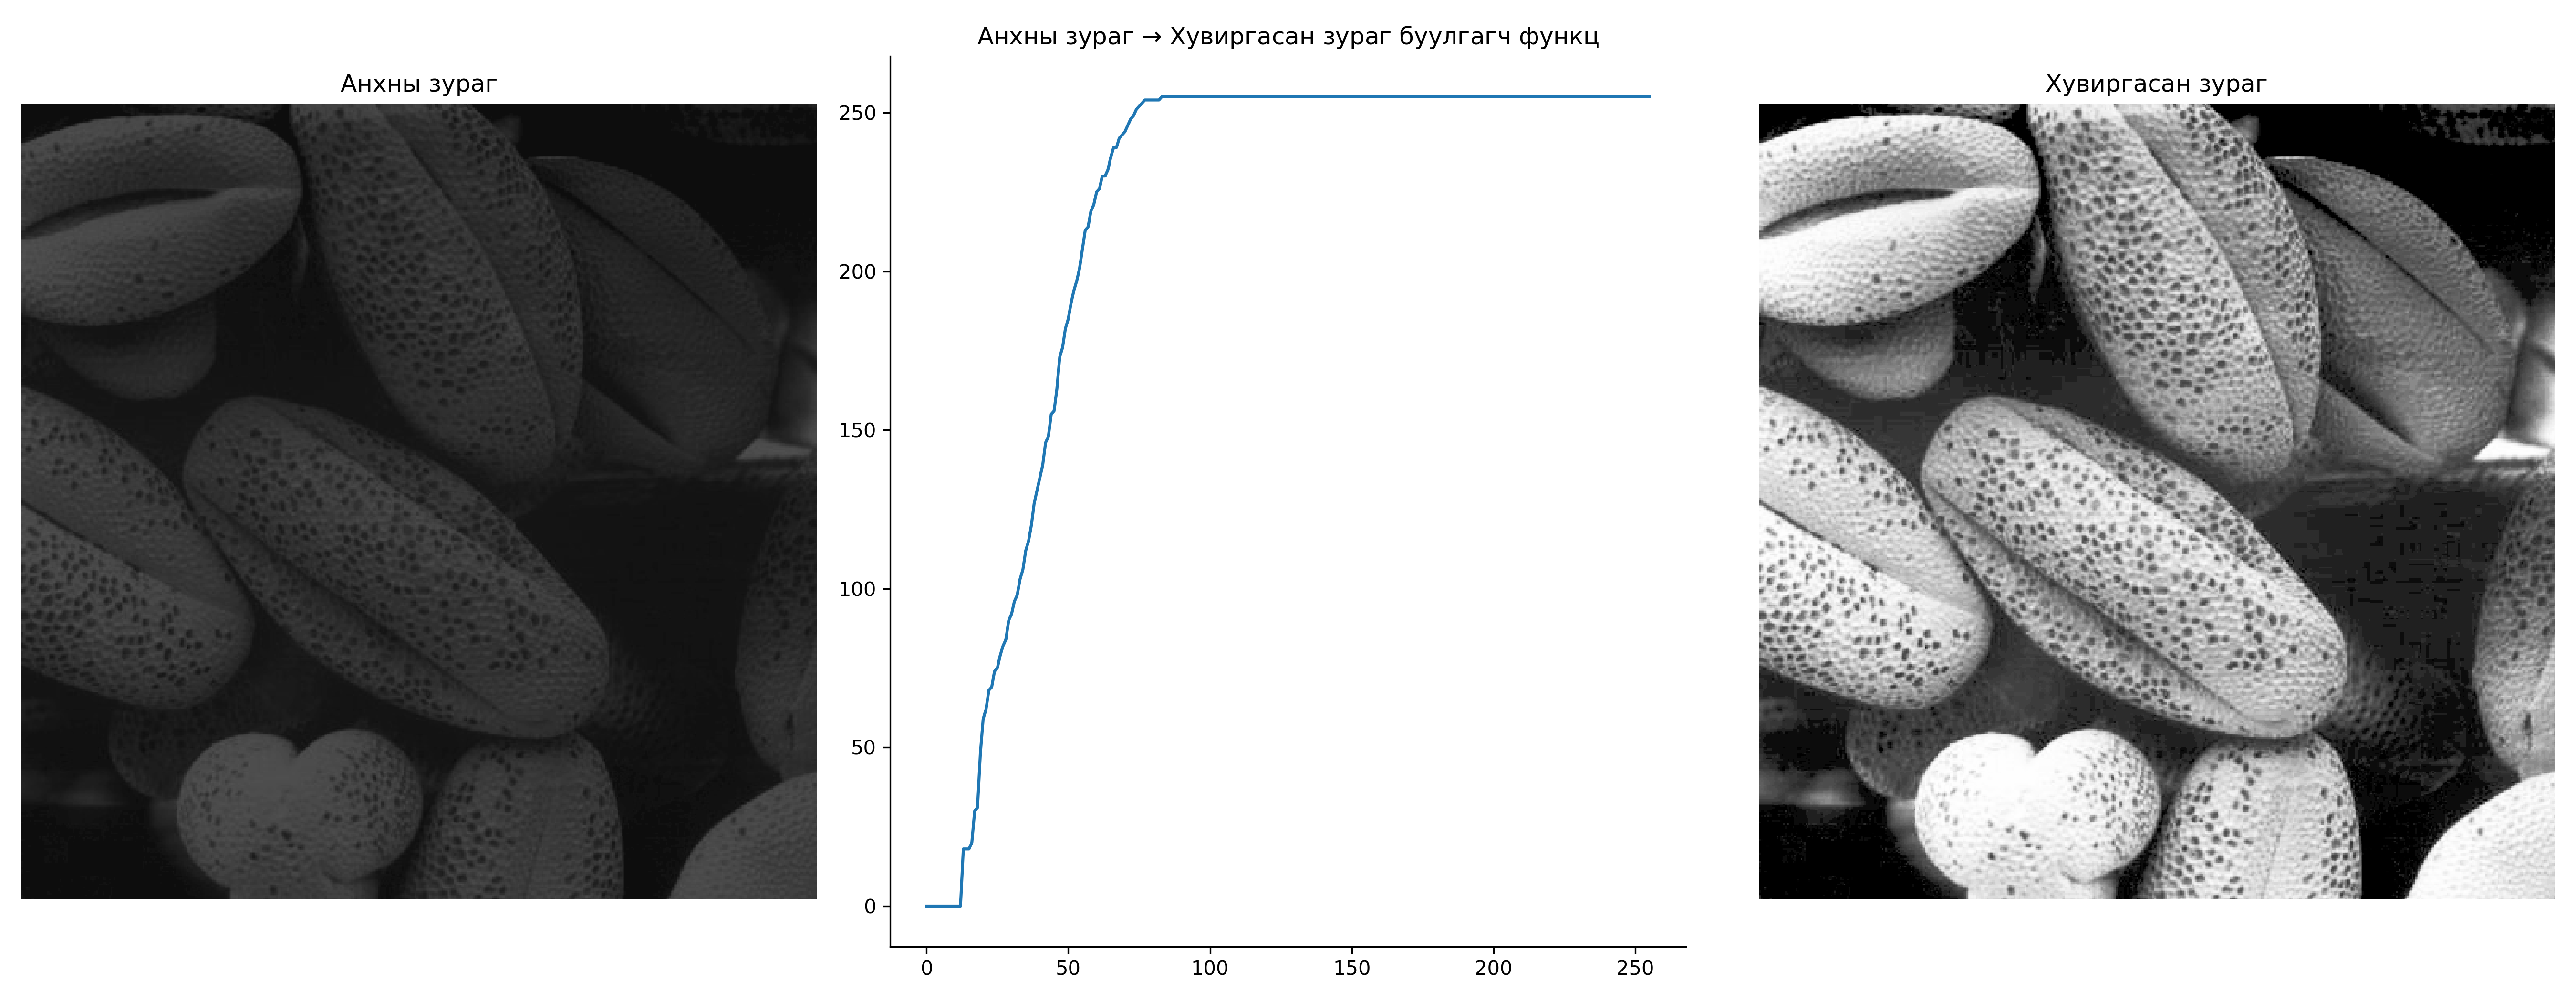
\includegraphics[scale = 0.30]{global_hist_eq_task_2.png}
  \caption[Intensity 1]{Гаралтын зураг ба буулгагч функц}
\end{figure}
\begin{figure}[H]
  \centering
  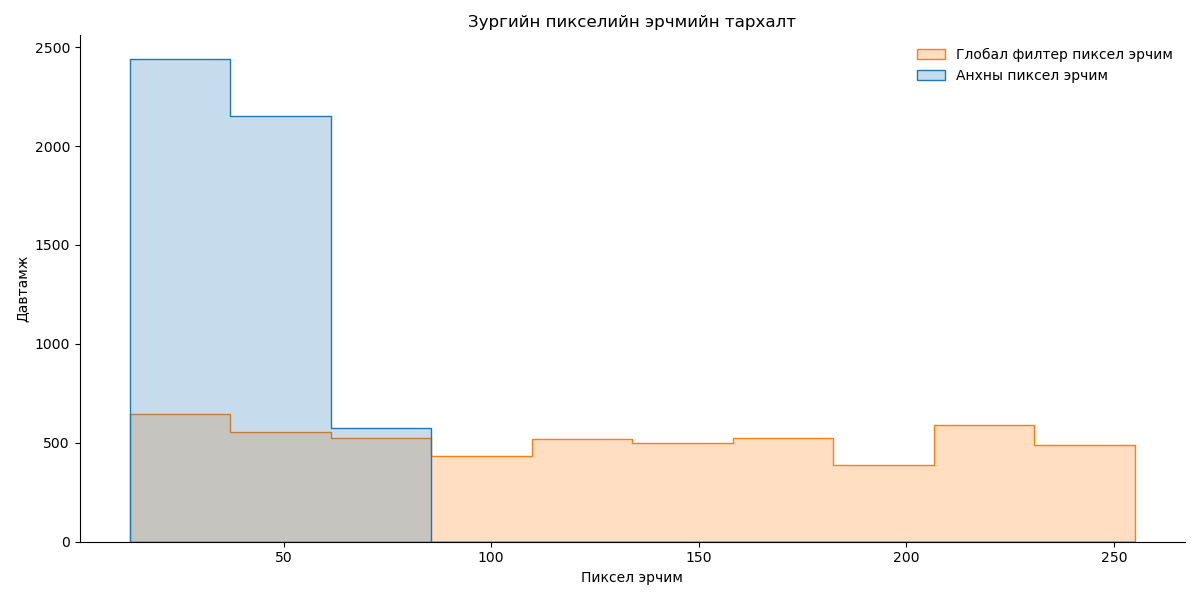
\includegraphics[scale = 0.30]{global_hist_eq_task_3.png}
  \caption[Intensity 1]{Оролтын болон гаралтын зургийн эрчмүүдийн тархалт}
\end{figure}
Одоо 4 ялгаатай эрчмийн тархалттай зургууд дээр уг аргыг ашигласан үр дүнг харуулъя. Энд зураг бүрийн эрчмийн тархалт нь голдуу зүүн эсвэл баруун хэсэгтээ буюу зургийн боломжит эрчим бүрийн хувьд жигд тархаагүй хэсэг газартаа бөөгнөрсөн хэв маягтай байсан.
\begin{figure}[H]
  \centering
  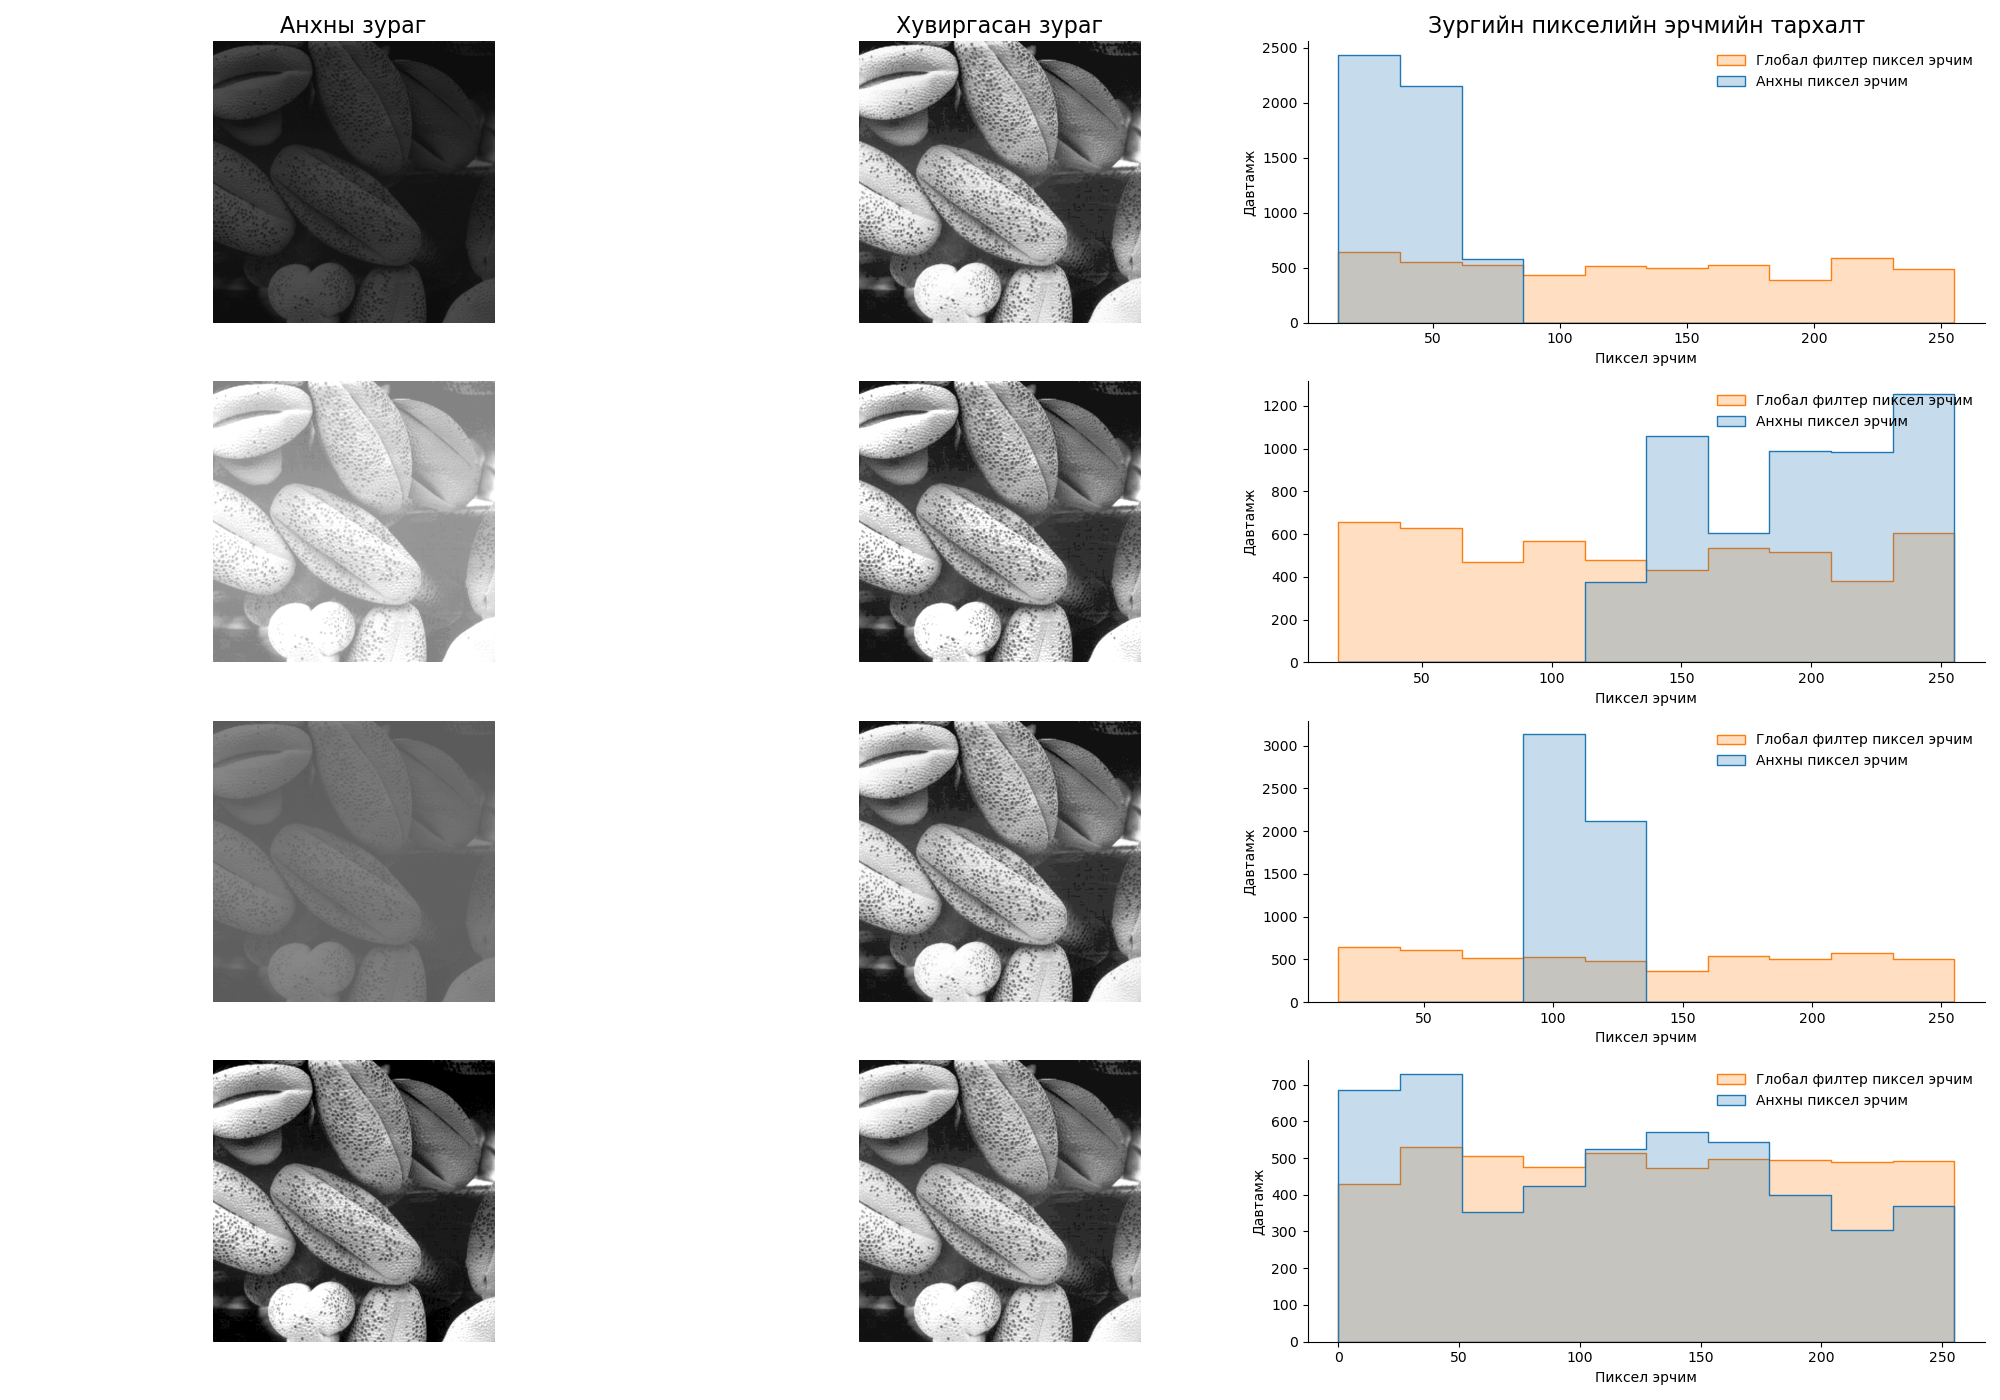
\includegraphics[scale = 0.30]{global_hist_eq_task_4.png}
  \caption[Intensity 1]{Ялгаатай эрчмийн тархалттай зургууд дээрх үр дүн}
\end{figure}
\begin{figure}[H]
  \centering
  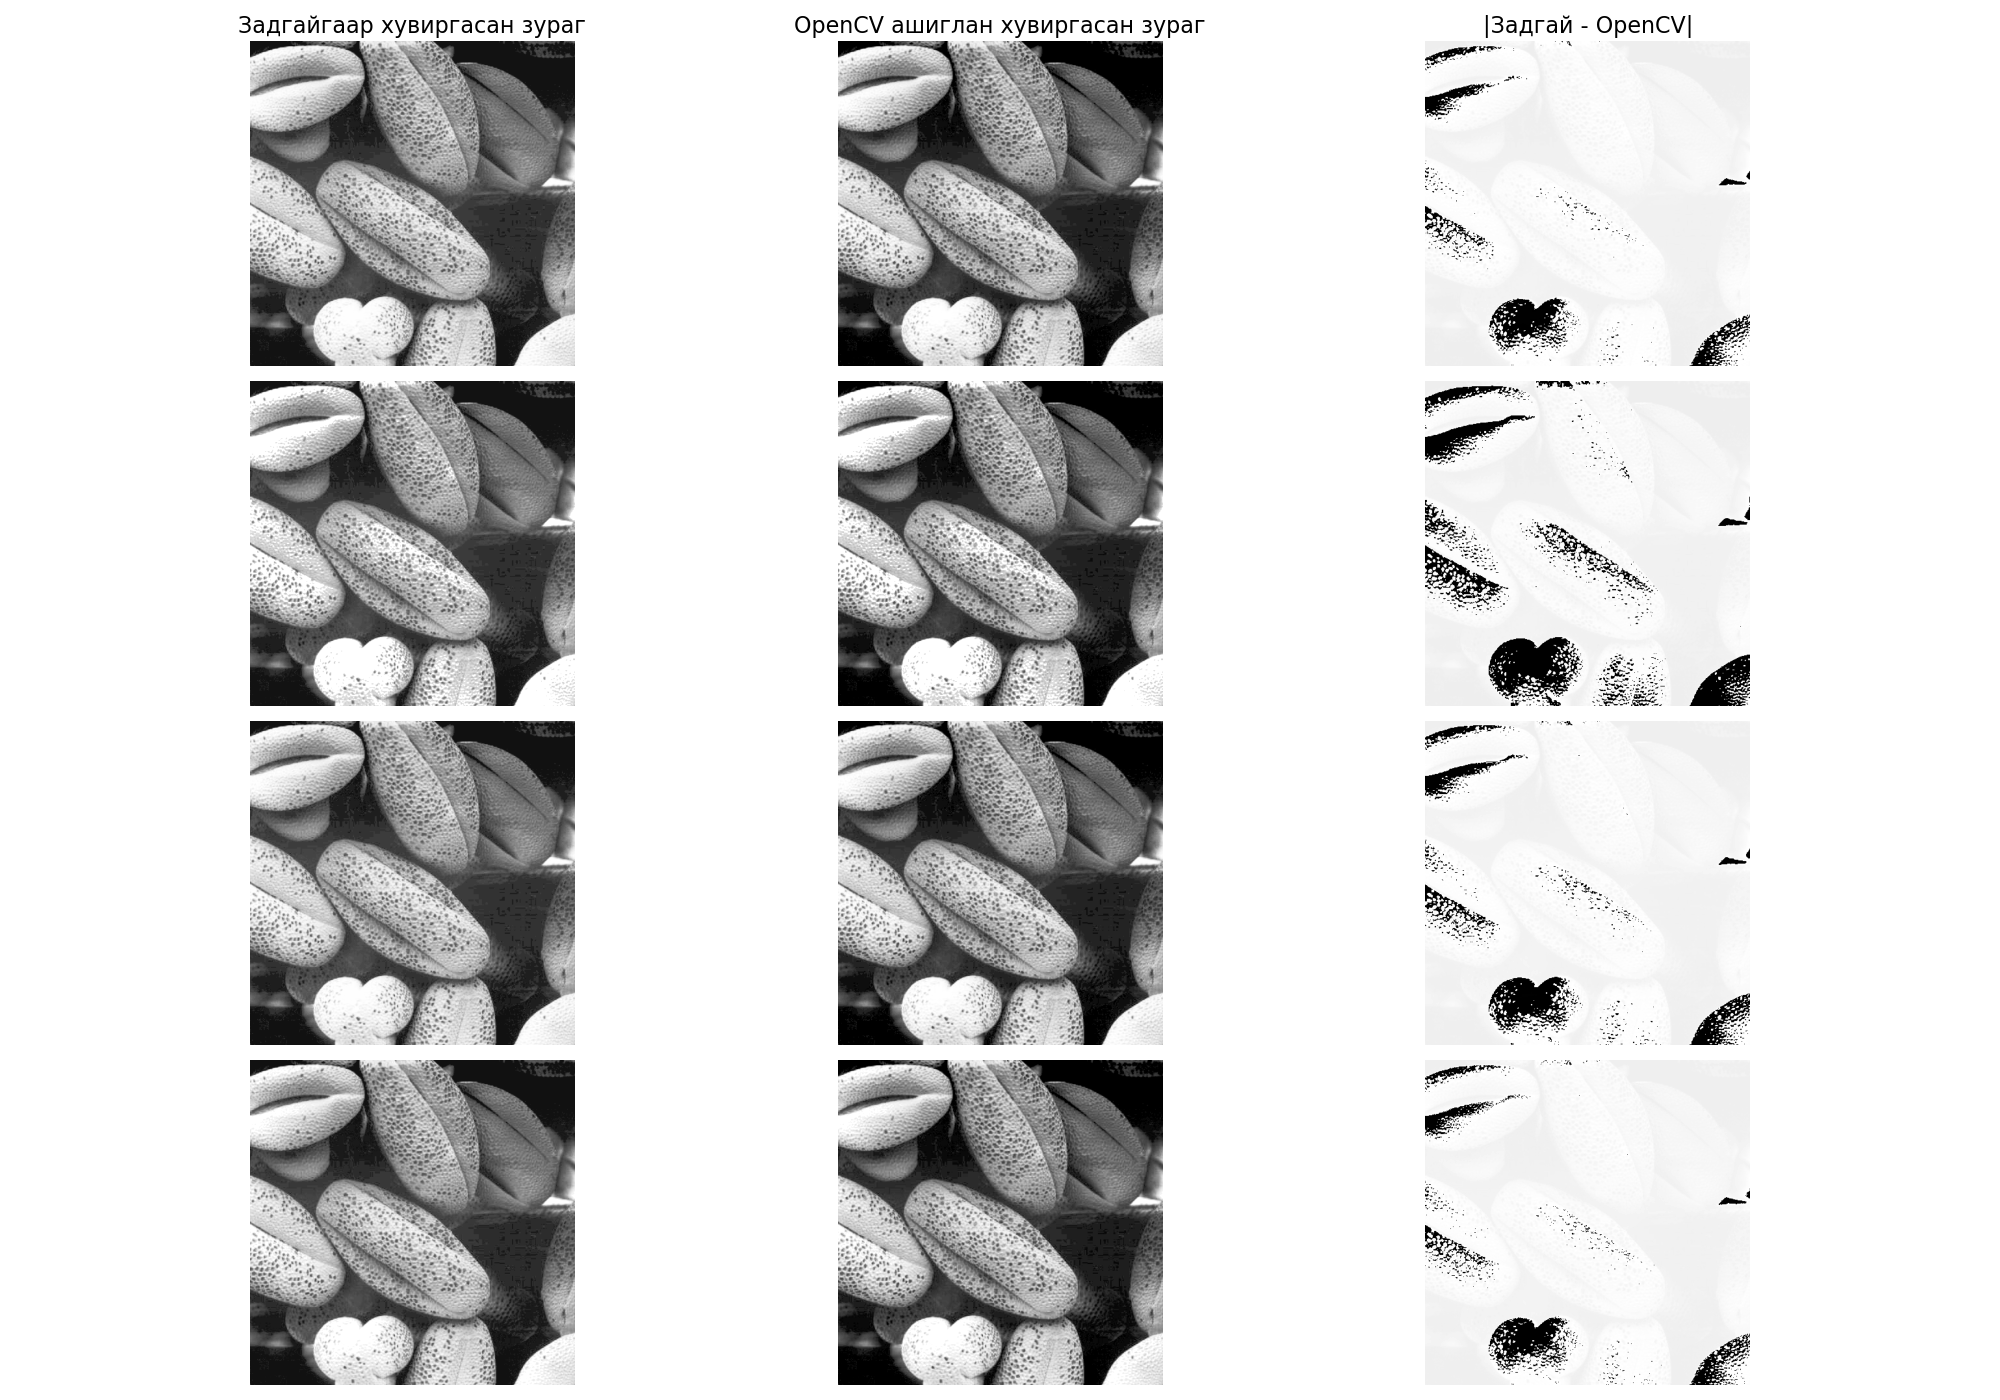
\includegraphics[scale = 0.30]{global_hist_eq_task_5.png}
  \caption[Intensity 1]{Гараар хувиргасан функц болон бэлэн функцийн ялгаа}
\end{figure}

Тэгэхээр сая бид зургийн эрчмийн тархалтыг нийтээр нь нормчлох аргын талаар үзсэн бол одоо хэсэг орчны хувьд нормчлох талаар үзье.
\begin{figure}[H]
  \centering
  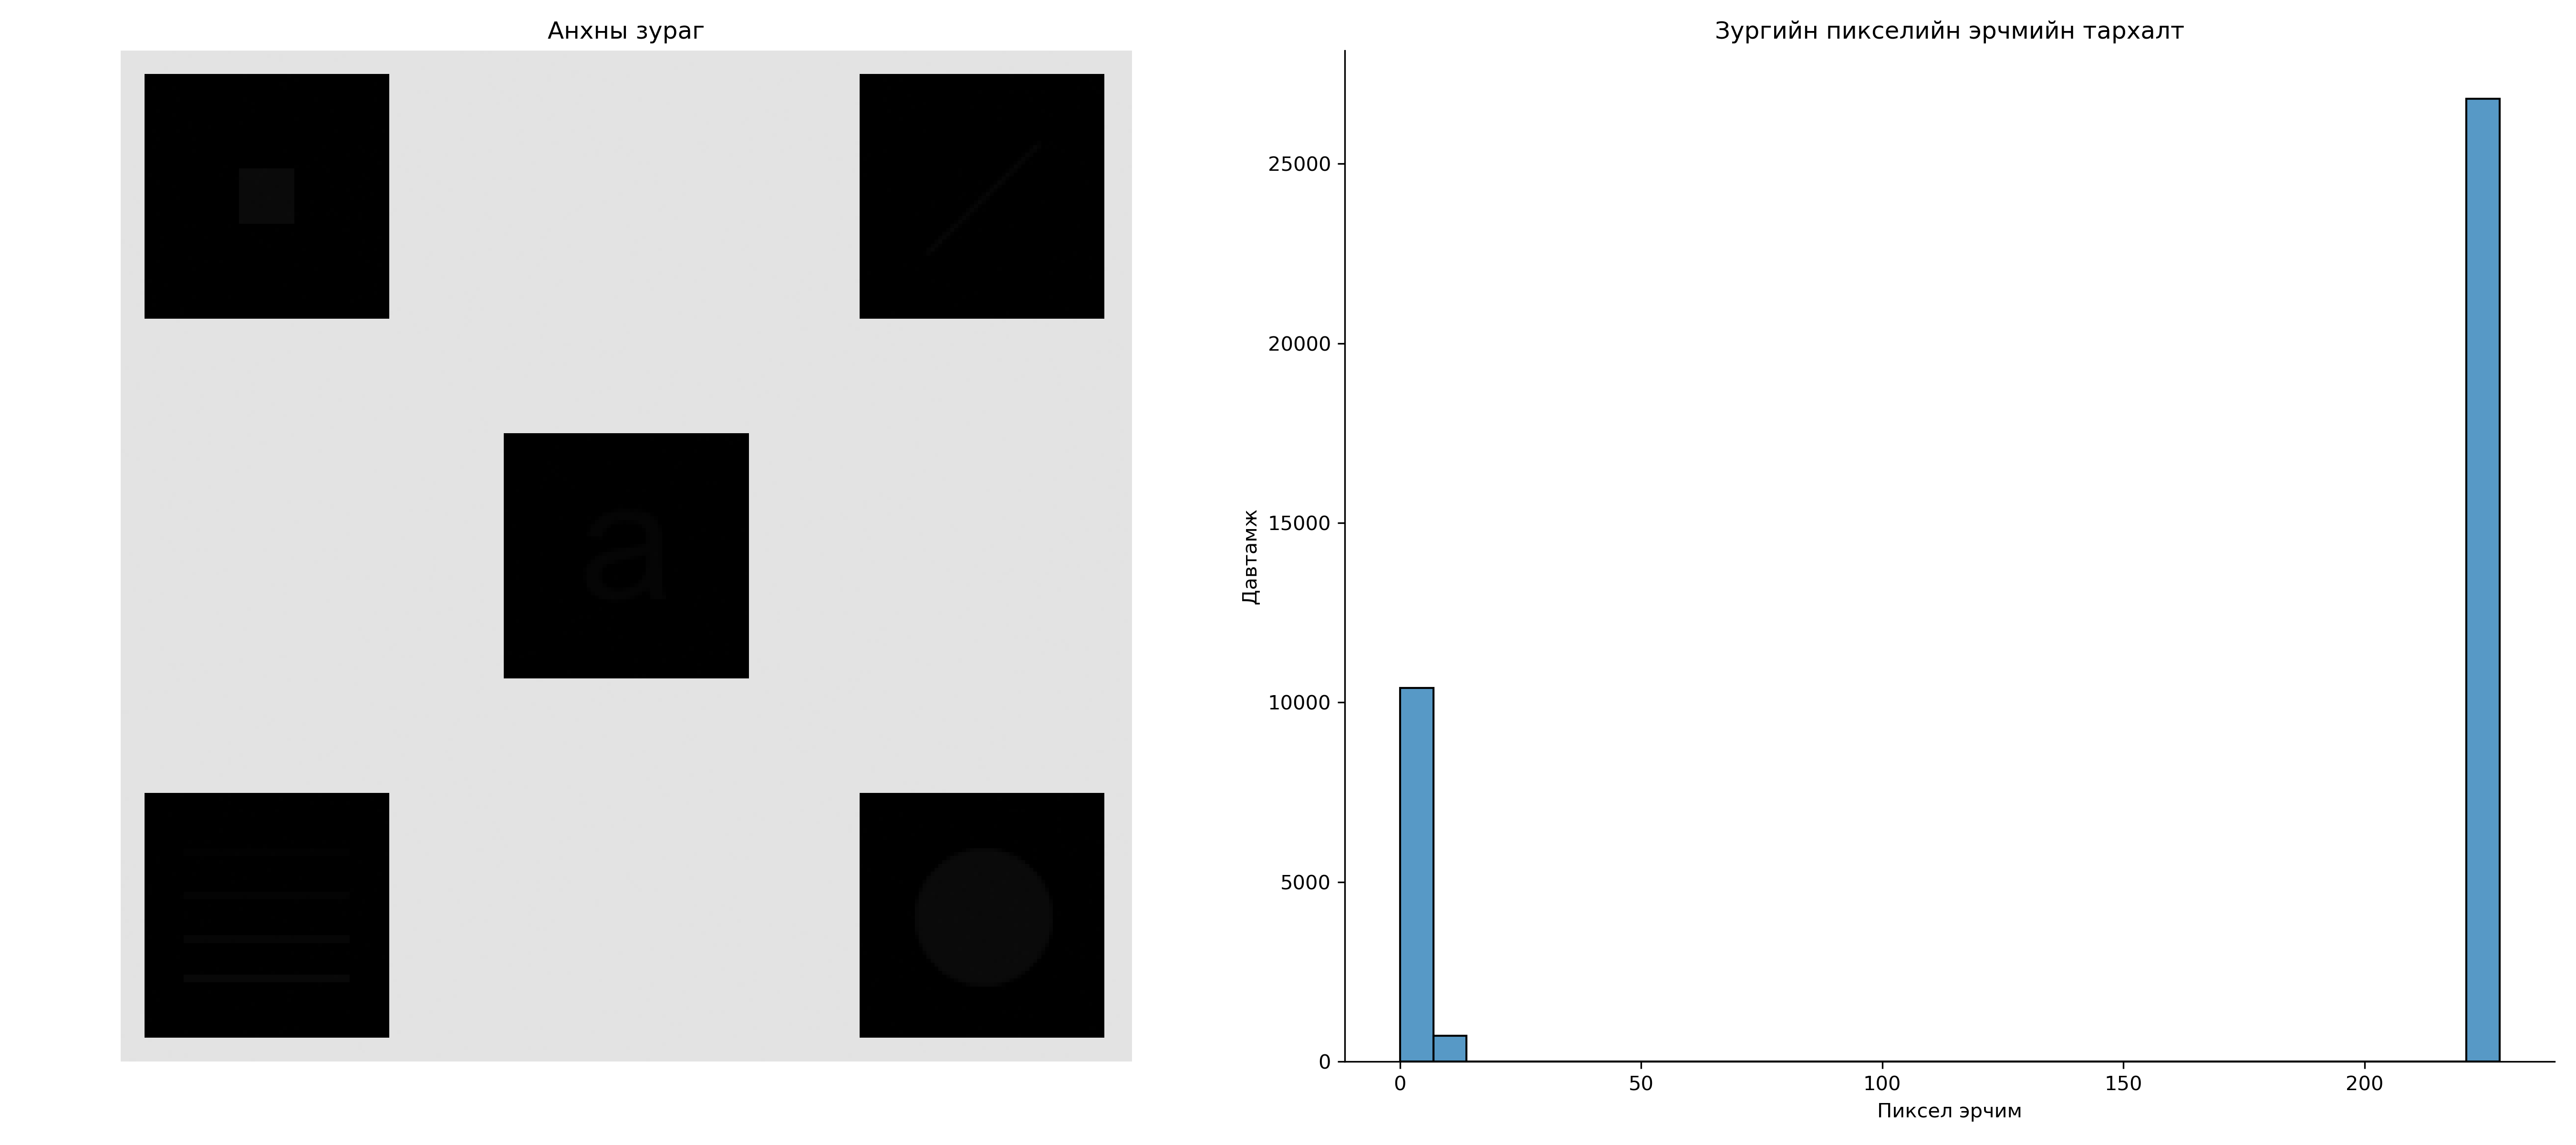
\includegraphics[scale = 0.30]{og_image.png}
  \caption[Intensity 1]{Оролтын зураг болон эрчмийн тархалт}
\end{figure}
Энэхүү зургийн хувьд глобал гистограм арга ашиглах нь дараах үг дүнг буцаана.
\begin{figure}[H]
  \centering
  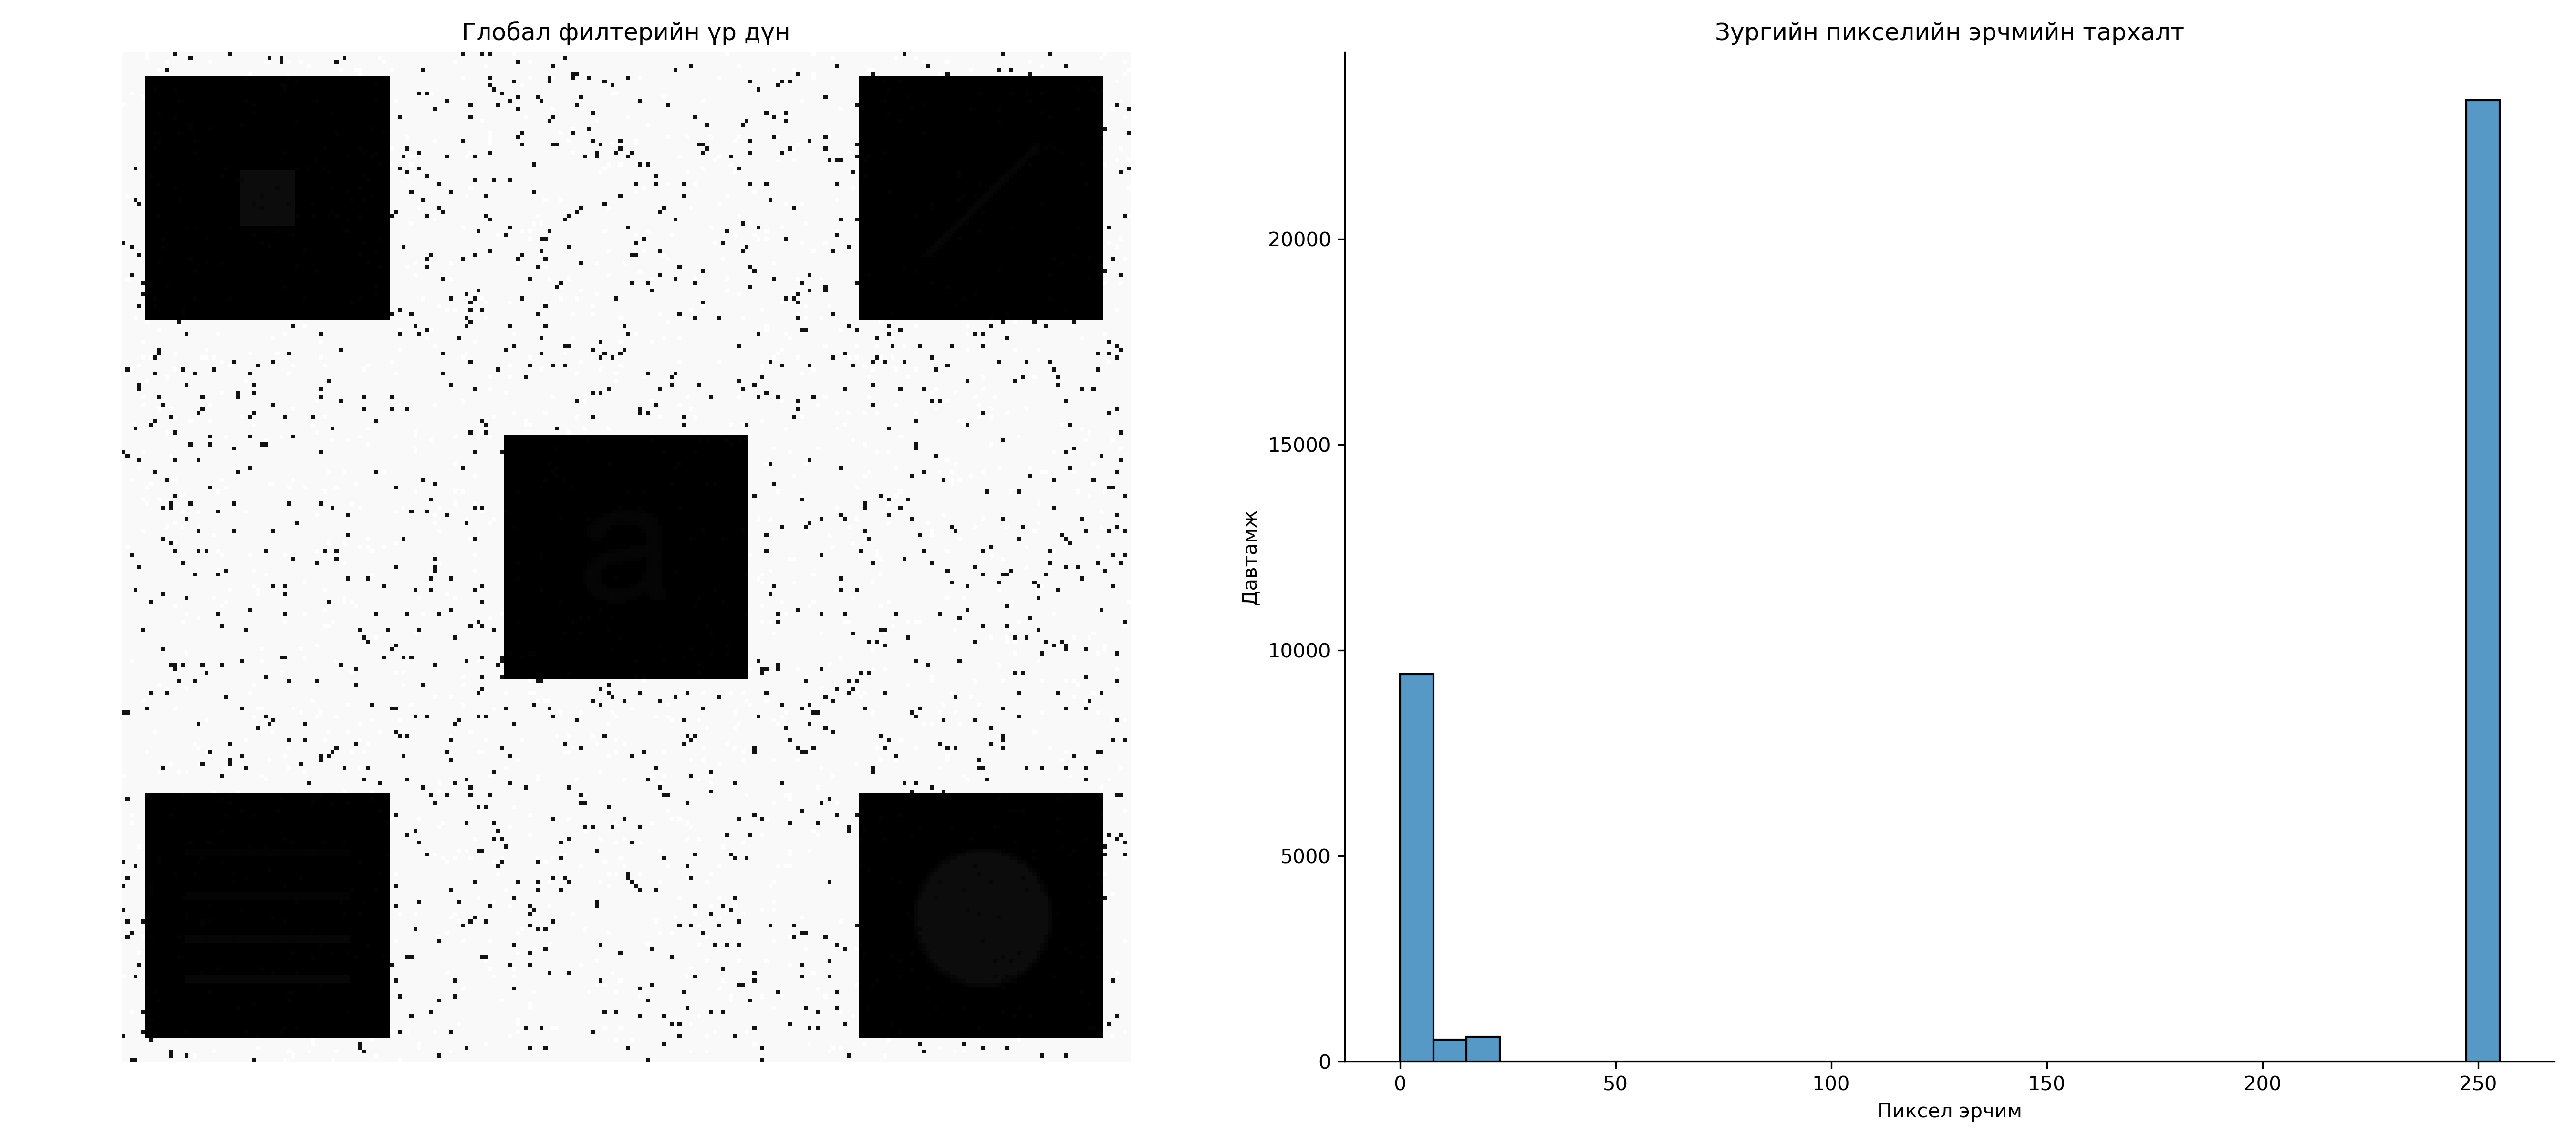
\includegraphics[scale = 0.30]{global_eq.png}
  \caption[Intensity 1]{Оролтын зургийн глобал гистограм аргын үр дүн}
\end{figure}
Энэхүү арга нь зургийн шуугианыг нэмэгдүүлсэн хэдий ч өөр хэрэгтэй мэдээлэл гаргаж чадахгүй байна. Учир нь бидэнд энэхүү зургаас хэрэгтэй байгаа пикселийн эрчим нь орчныхоо эсвэл нийт зургийн эрчимтэй харьцуулахад нөлөө багатай гэж үзэж нийт зургийн хувьд гистограм арга ашиглах биш харин хэсэг орчны хувьд ашиглая.
\begin{figure}[H]
  \centering
  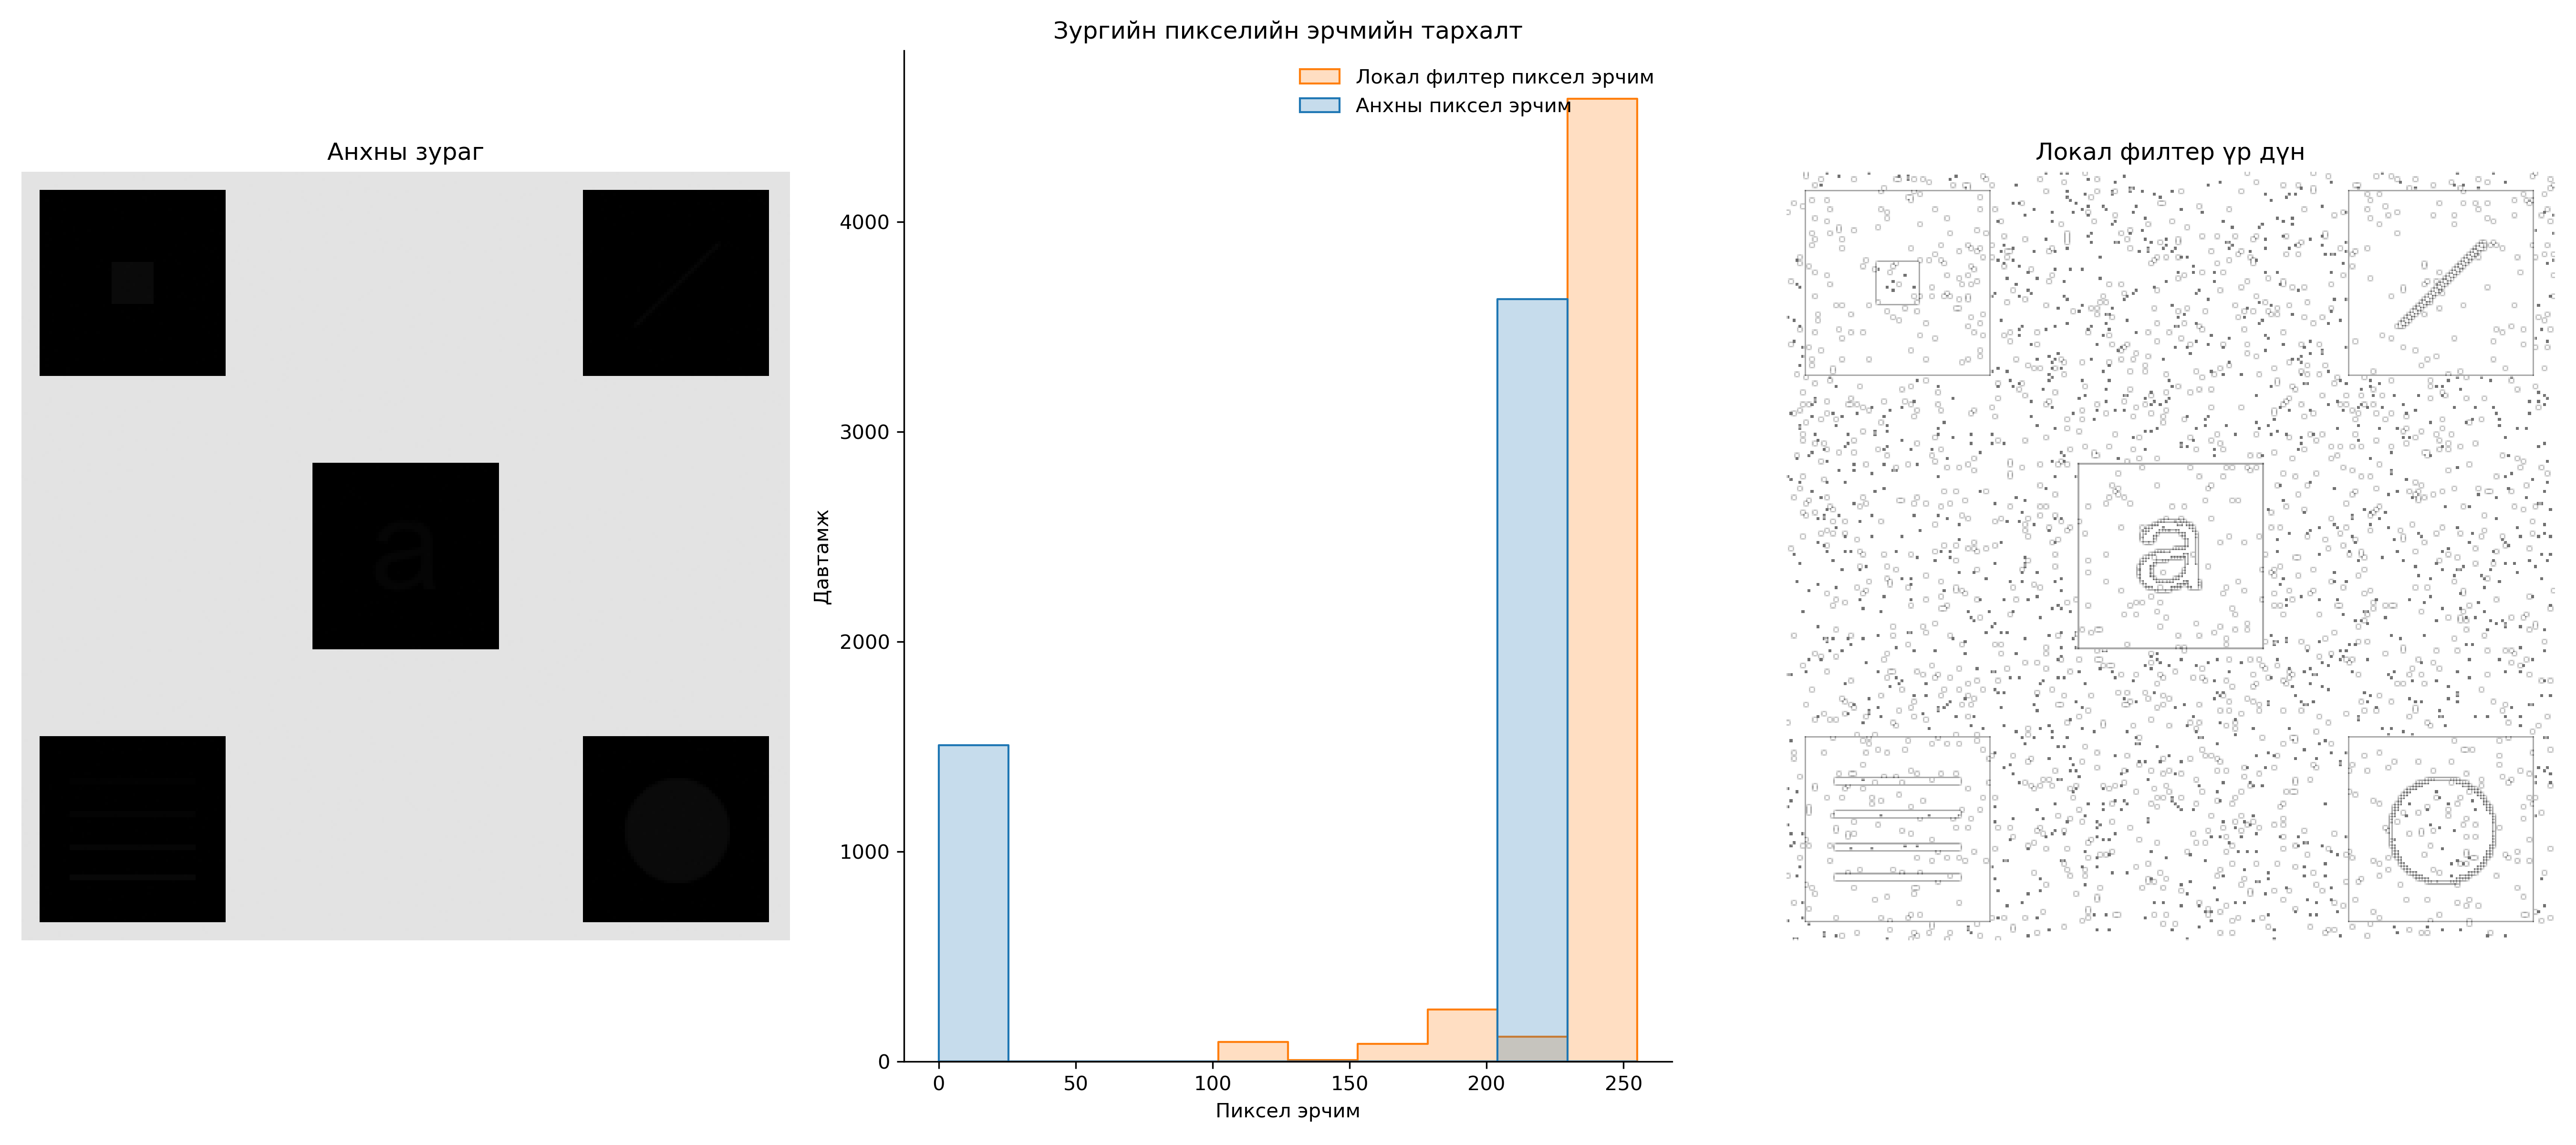
\includegraphics[scale = 0.30]{local_eq_1.png}
  \caption[Intensity 1]{Оролтын зургийн орчны хувьд гистограм арга ашигласан үр дүн}
\end{figure}
\begin{python}
def local_hist_eq(img, mask_size, stride = 1):
    height, width = img.shape
    mask_iter = mask_size // 2
    enhanced_image = np.zeros((height, width), dtype = np.uint8)

    padding = mask_iter * stride
    padded_img = np.pad(img, pad_width = ((padding, padding), (padding, padding)), 
                        mode = 'constant', constant_values = 0)

    for i in range(mask_iter, height + mask_iter, stride):
        for j in range(mask_iter, width + mask_iter, stride):
            neighborhood = padded_img[i - mask_iter: i + mask_iter + 1, j - mask_iter: j + mask_iter + 1]
            hist = np.histogram(neighborhood, bins = np.arange(256))[0]
            cdf = hist.cumsum()

            if neighborhood.shape[1] <= mask_iter:
                enhanced_pixel = cdf[neighborhood[mask_iter, 0]] * 255 / cdf[-1]
            elif neighborhood.shape[0] <= mask_iter:
                enhanced_pixel = cdf[neighborhood[0, mask_iter]] * 255 / cdf[-1]
            else:
                enhanced_pixel = cdf[neighborhood[mask_iter, mask_iter]] * 255 / cdf[-1]
            enhanced_image[i-mask_iter, j-mask_iter] = enhanced_pixel
            
    return enhanced_image
\end{python} 
\begin{python}
img = Image.open(f"{img_dir}/Fig0326(a)(embedded_square_noisy_512).tif")
img = np.asarray(img)

enhanced_image = local_hist_eq(img, 3, stride = 1)
\end{python} \hfill \break\hfill \break
Дээрх зурагт $3\times3$ маскийг 1 пикселийн зайтай шилжүүлж байсан бол одоо $5\times5$ маскийг 1-с олон пикселийн зайтай шилжүүлэх процесс хэрхэн харагдахыг сонирхъё.
\begin{python}
def stride_viz(height, width, stride, mask_size):
    iter_cnt = 0
    mask_iter = mask_size // 2
    img = np.zeros((height, width))

    for i in range(mask_iter, height + mask_iter, stride):
        for j in range(mask_iter, width + mask_iter, stride):
            img[i - mask_iter: i + mask_iter + 1, j - mask_iter: j + mask_iter + 1] = 1
            iter_cnt += 1
    
    return img, iter_cnt

height, width = (100, 100)
img_1, iter_cnt_1 = stride_viz(height, width, stride = 1, mask_size = 5)
img_2, iter_cnt_2 = stride_viz(height, width, stride = 3, mask_size = 5)
img_3, iter_cnt_3 = stride_viz(height, width, stride = 5, mask_size = 5)
img_4, iter_cnt_4 = stride_viz(height, width, stride = 7, mask_size = 5)
img_5, iter_cnt_5 = stride_viz(height, width, stride = 8, mask_size = 5)
img_6, iter_cnt_6 = stride_viz(height, width, stride = 11, mask_size = 5)
\end{python} 
\begin{figure}[H]
  \centering
  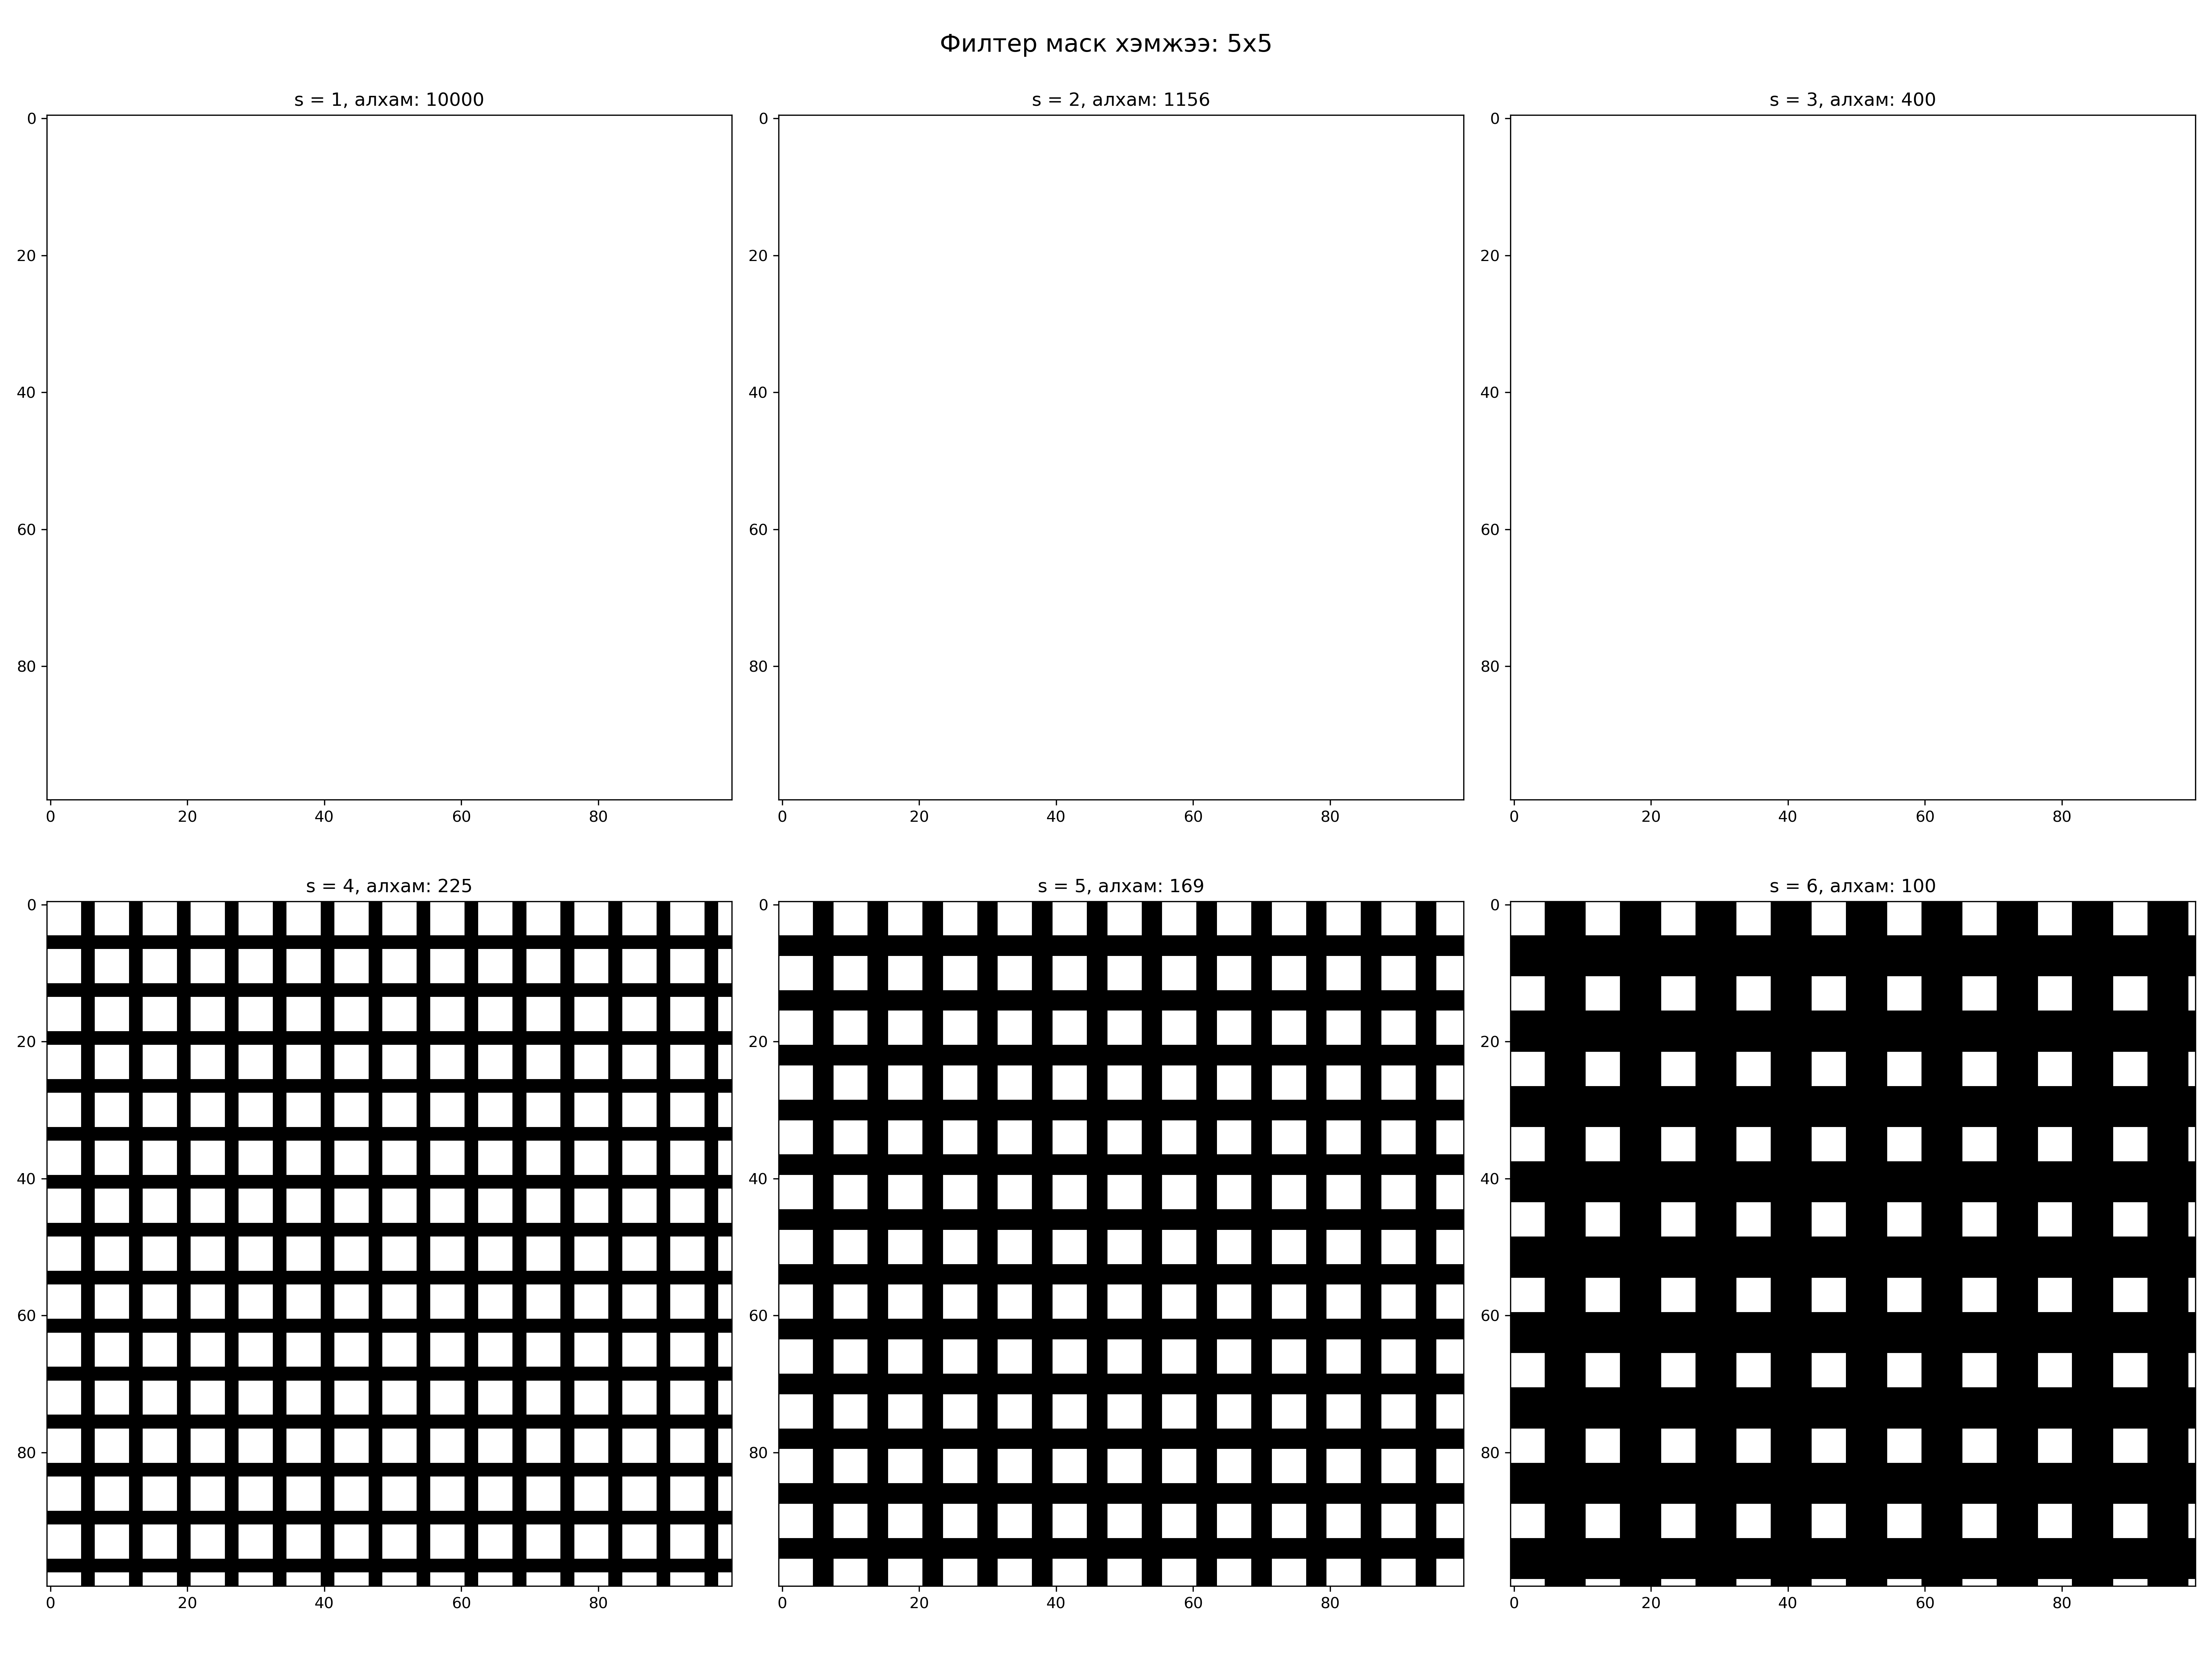
\includegraphics[scale = 0.30]{mask_stride_size.png}
  \caption[Intensity 1]{$5\times5$ маск ялгаатай зайгаар шилжүүлэх нь}
\end{figure}
Одоо тэгвэл оролтын зургийн хувьд ялгаатай зайгаар маск шилжүүлэхэд үүсэх зургийг сонирхъё.
\begin{figure}[H]
  \centering
  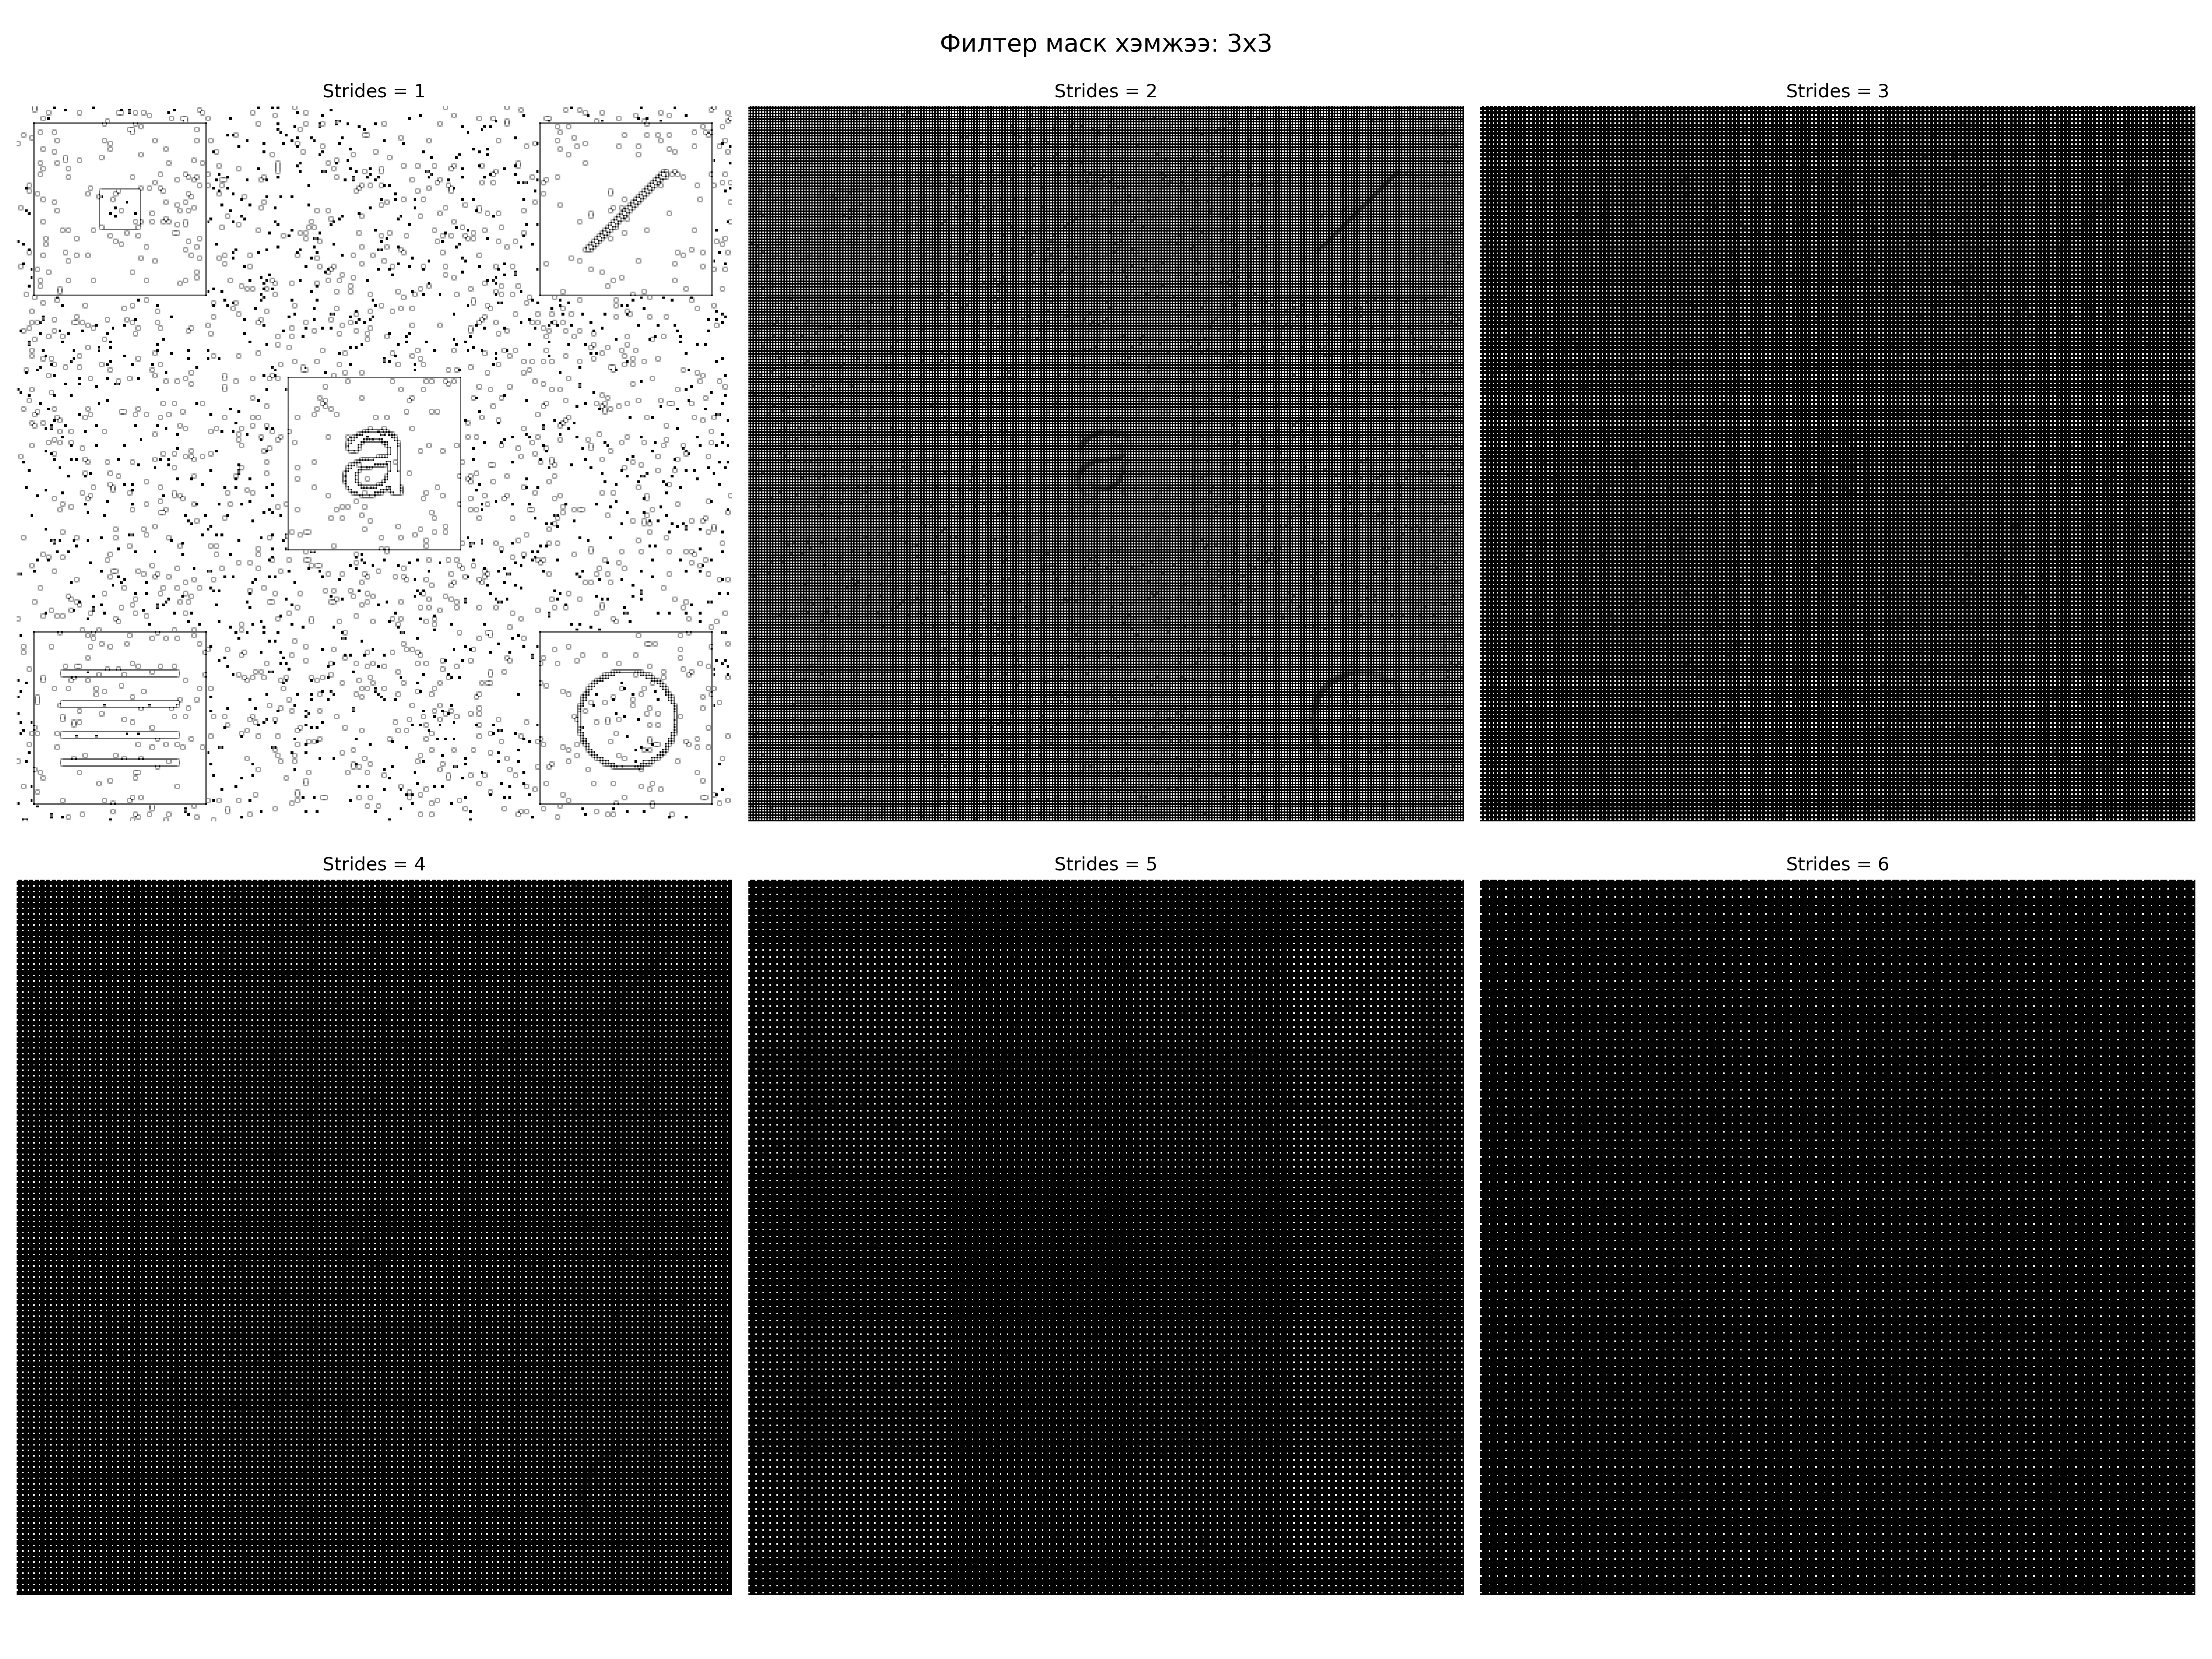
\includegraphics[scale = 0.30]{mask_3_strides.png}
  \caption[Intensity 1]{Оролтын зургийн хувьд маск ялгаатай зайгаар шилжүүлэх нь}
\end{figure}
Эндээс $Strides = 1, 2, 3$ хувьд үүсэх зургийн тархалтуудыг харъя.
\begin{figure}[H]
  \centering
  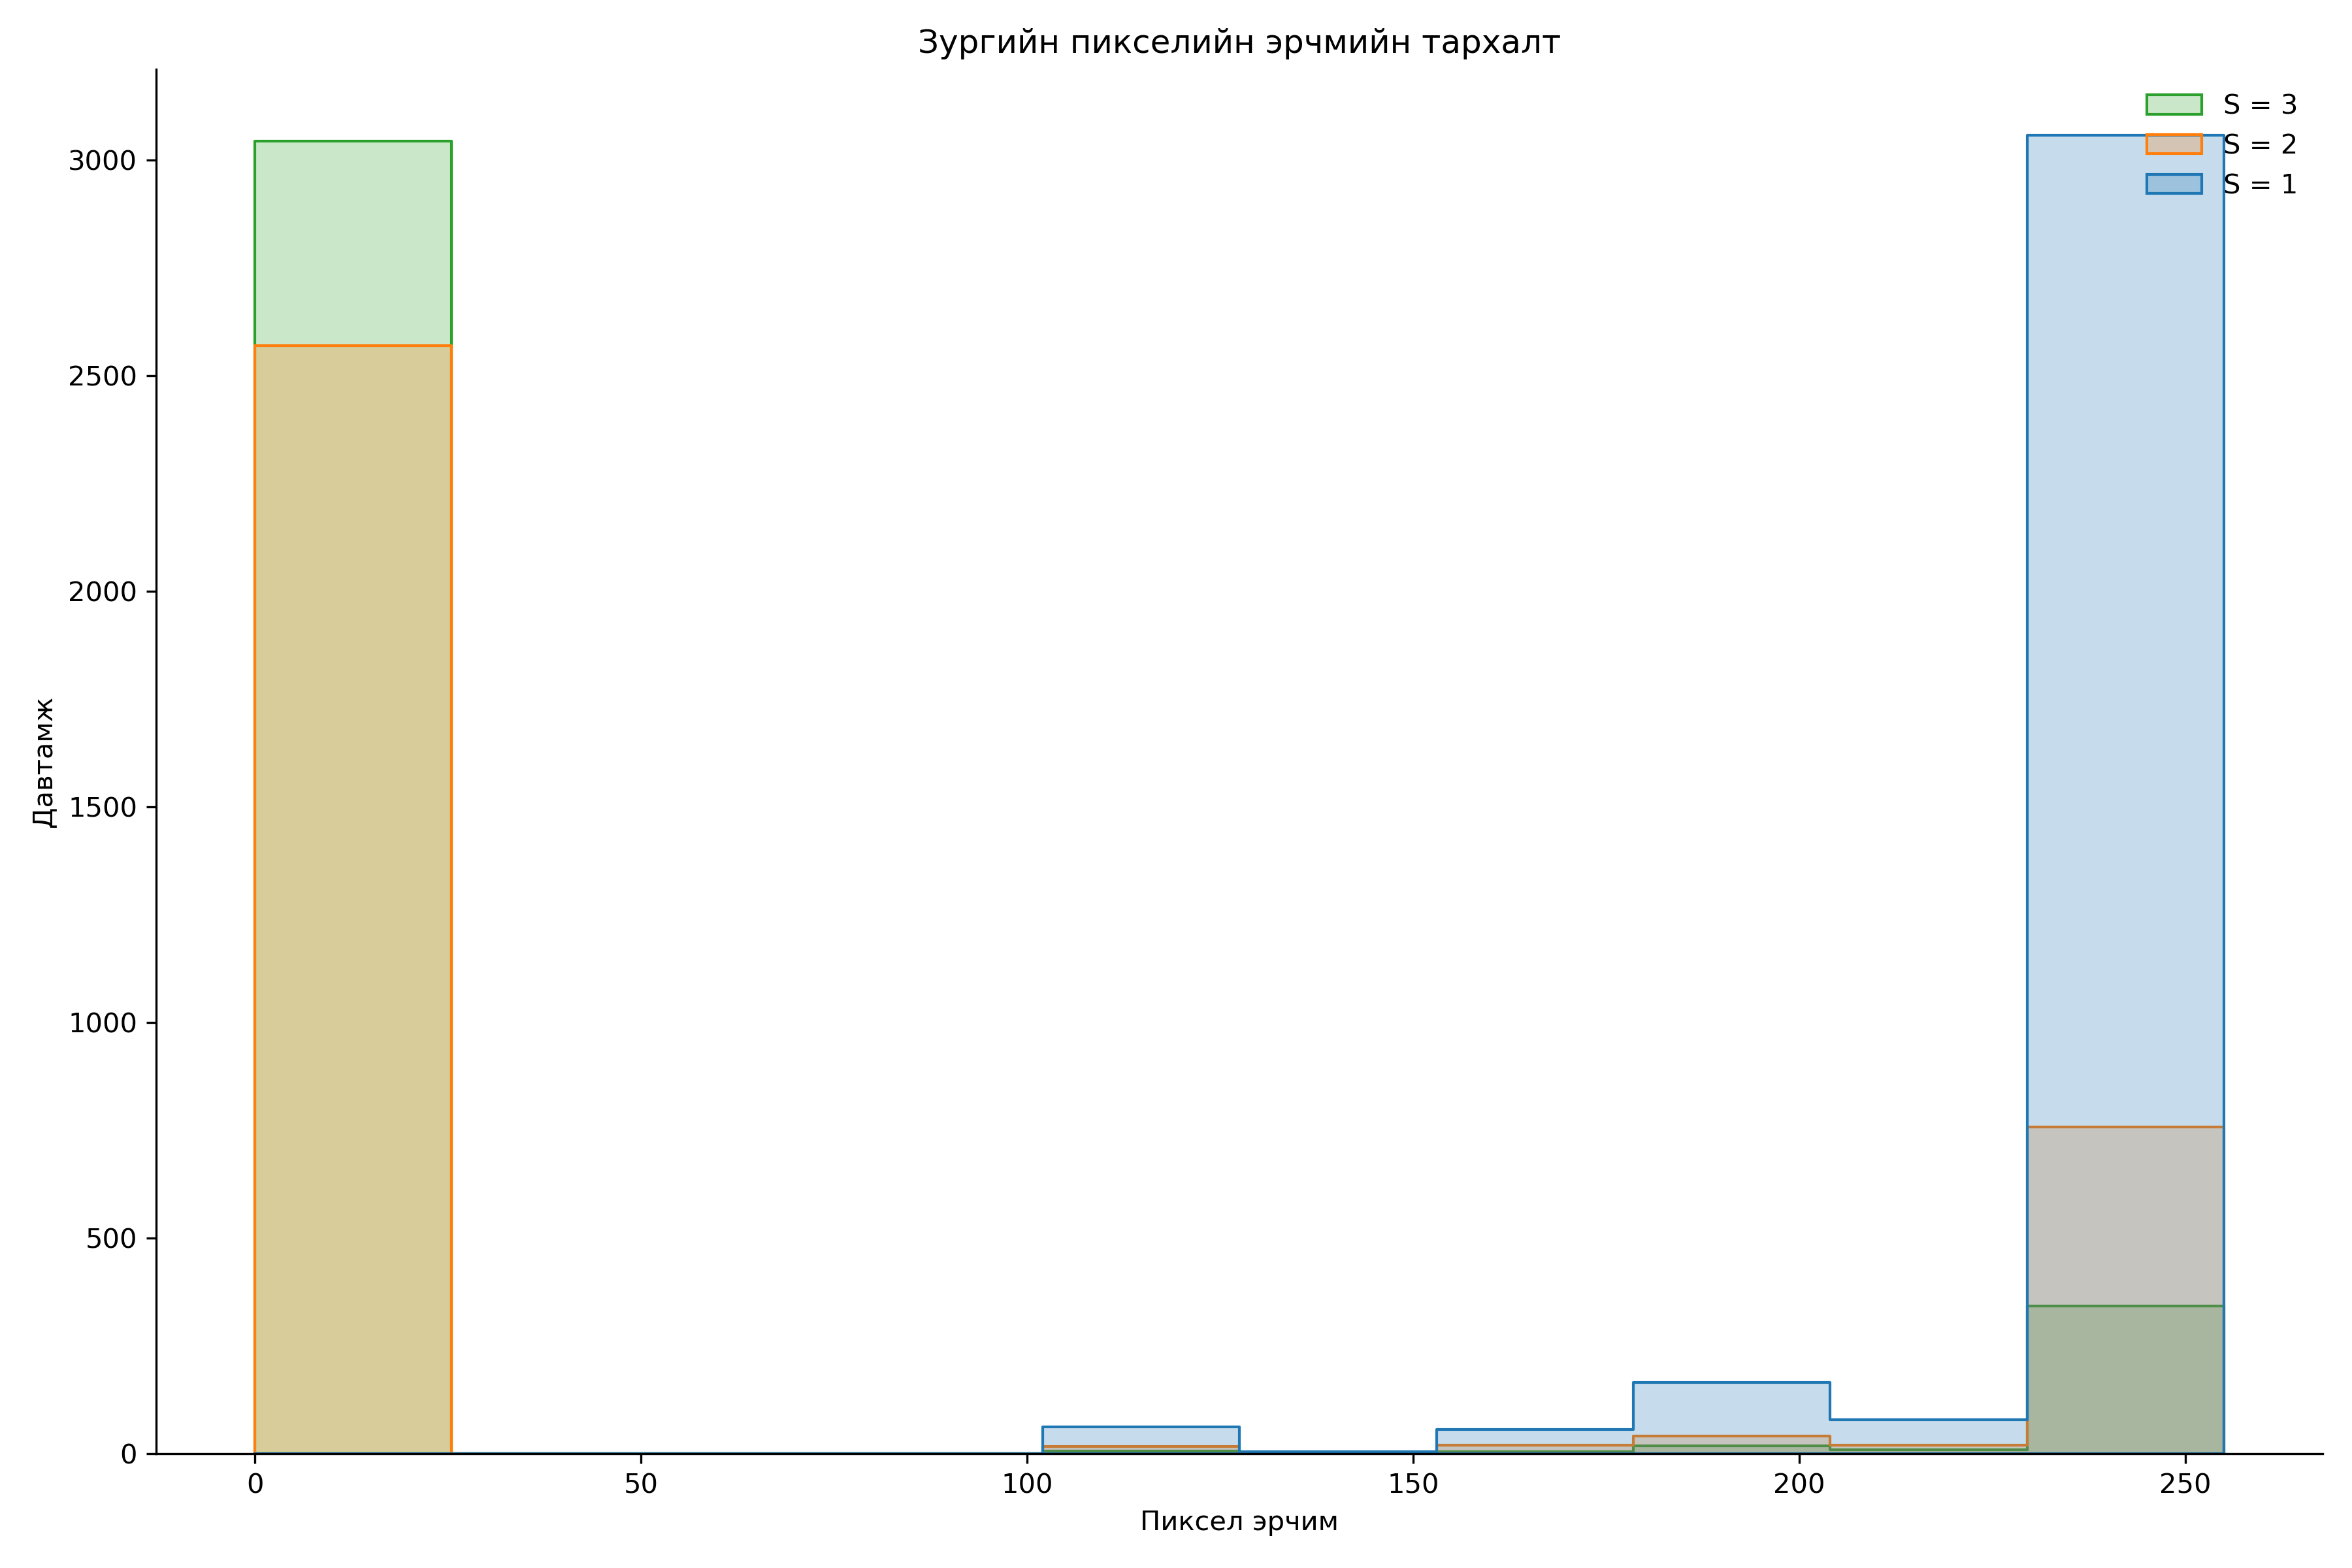
\includegraphics[scale = 0.30]{img_strides_hist.png}
  \caption[Intensity 1]{Оролтын зургийн хувьд маскийг 1, 2, 3 зайгаар шилжүүлсэн нь}
\end{figure}

Одоо харин маскийн хэмжээг өөрчилж үзье.
\begin{figure}[H]
  \centering
  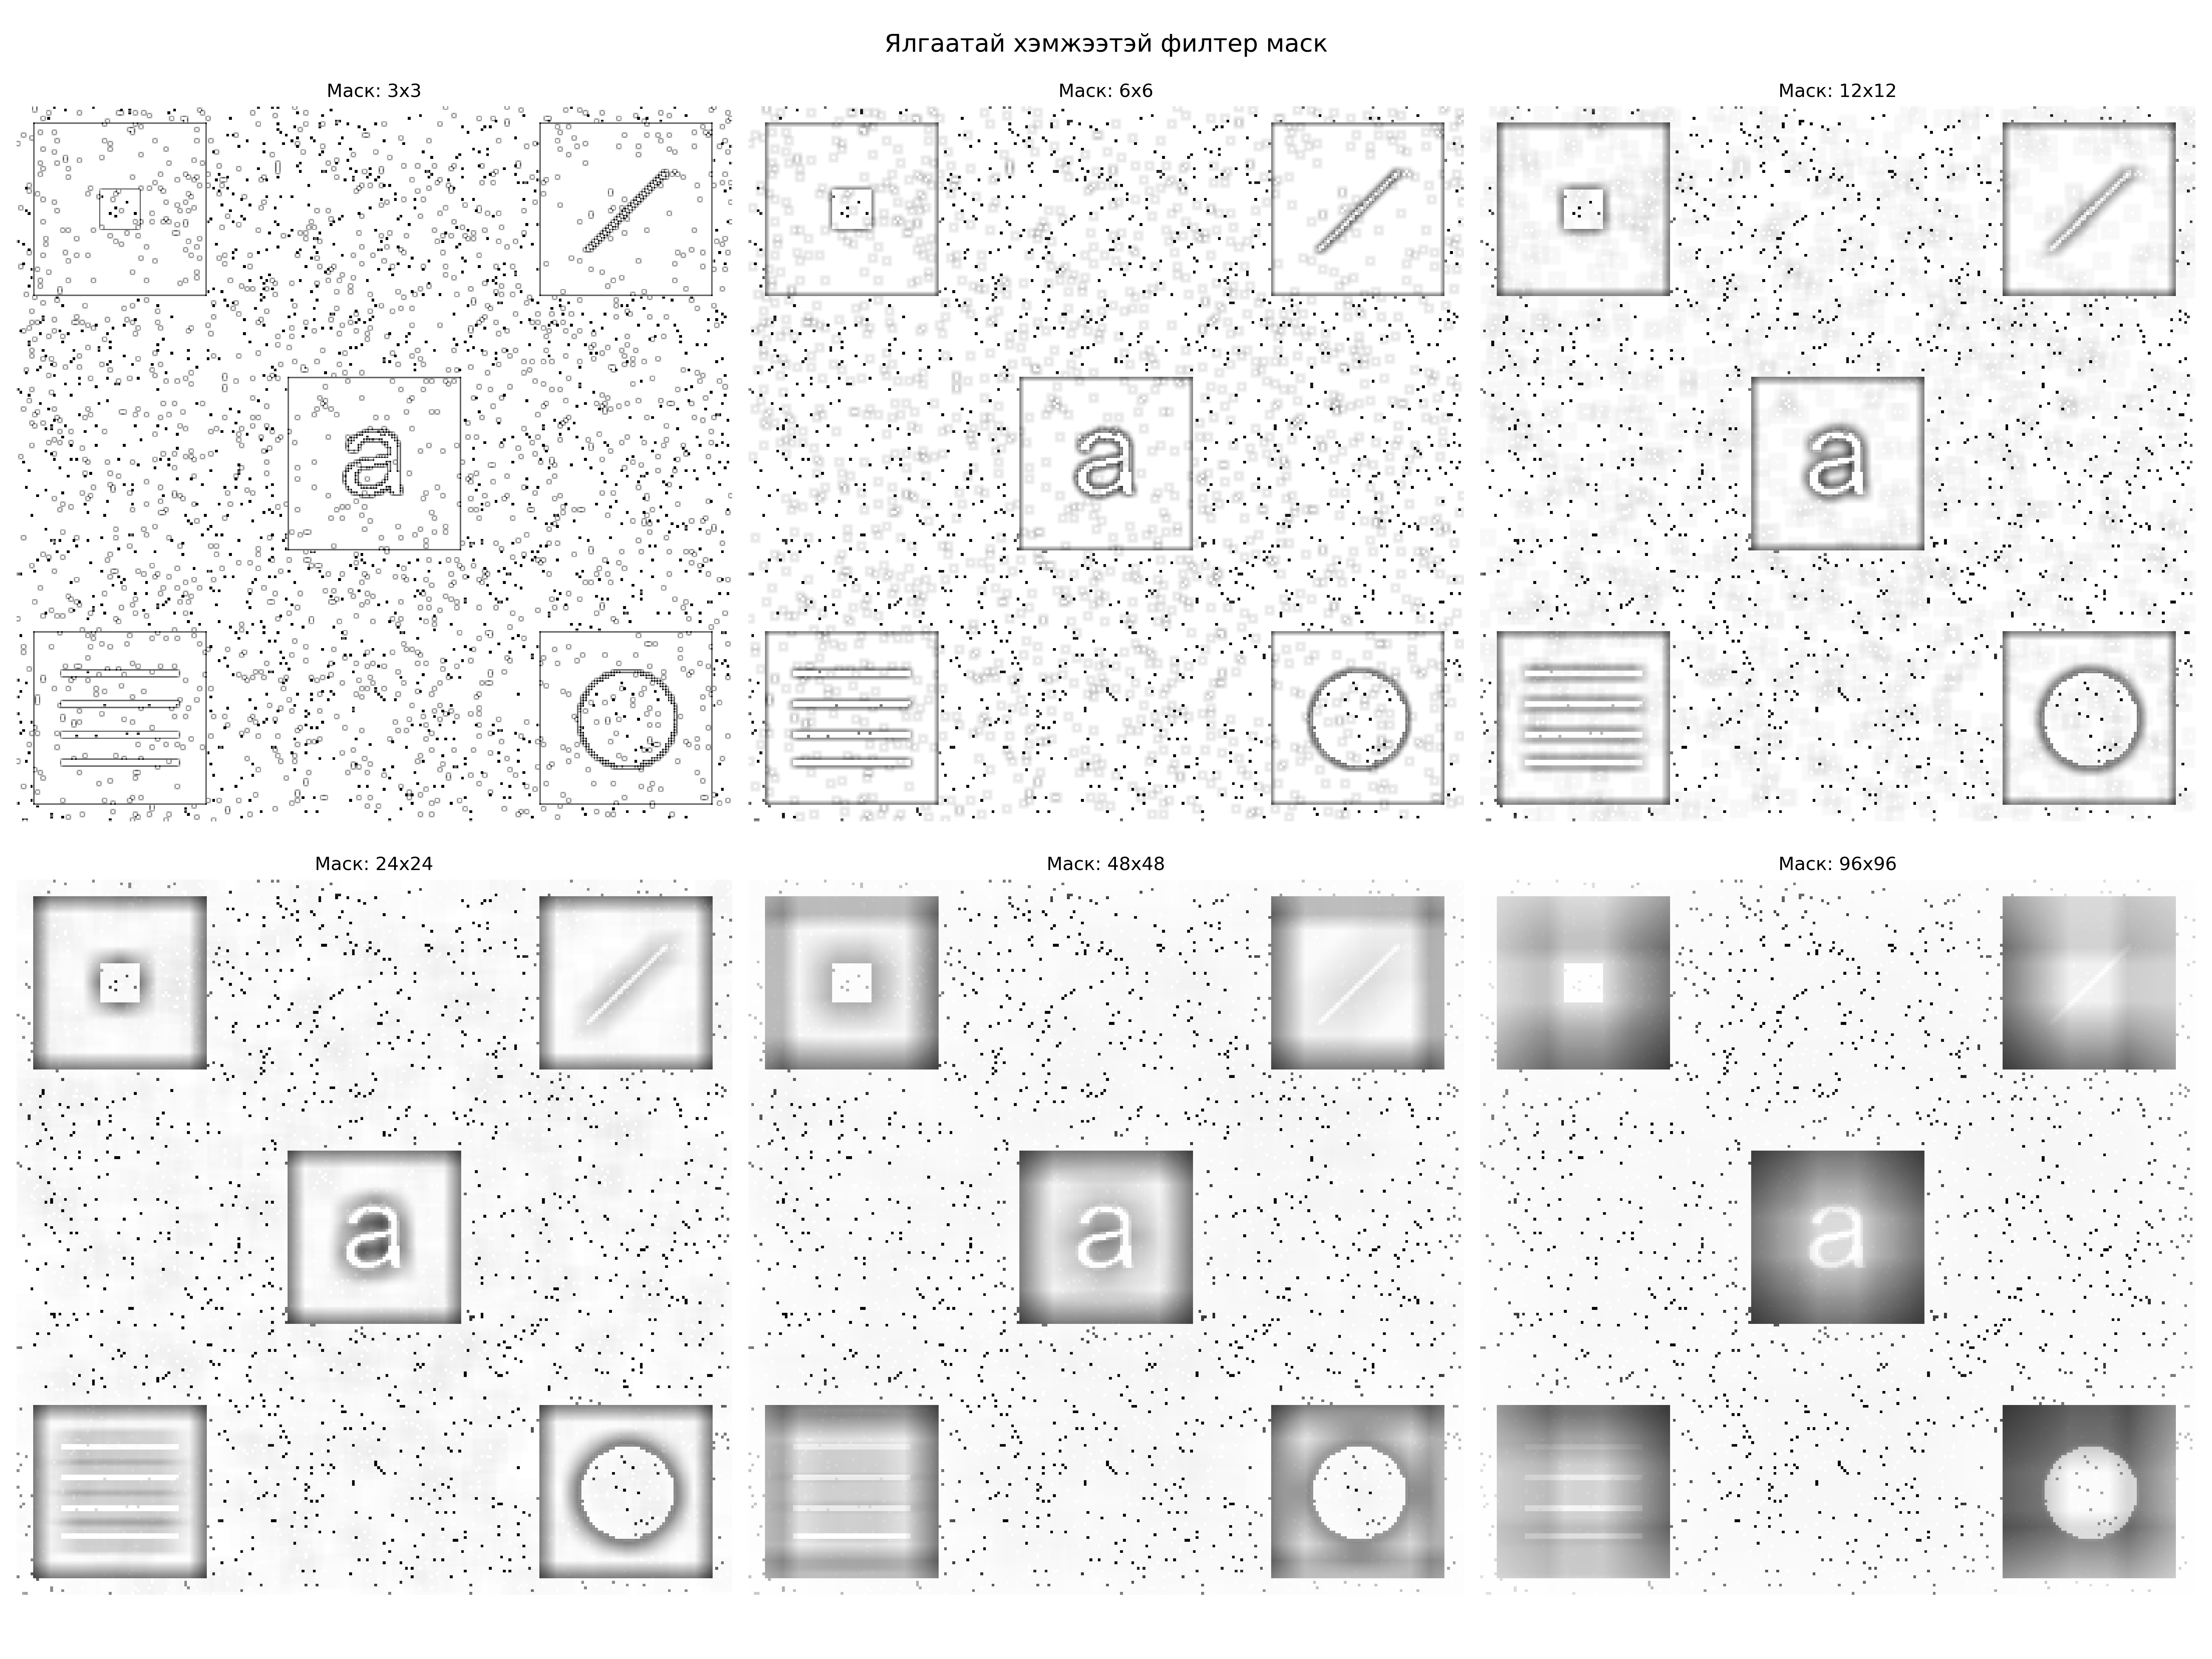
\includegraphics[scale = 0.30]{mask_different_strides_1.png}
  \caption[Intensity 1]{Оролтын зургийн хувьд маскийг өөрчилсөн нь}
\end{figure}
\begin{figure}[H]
  \centering
  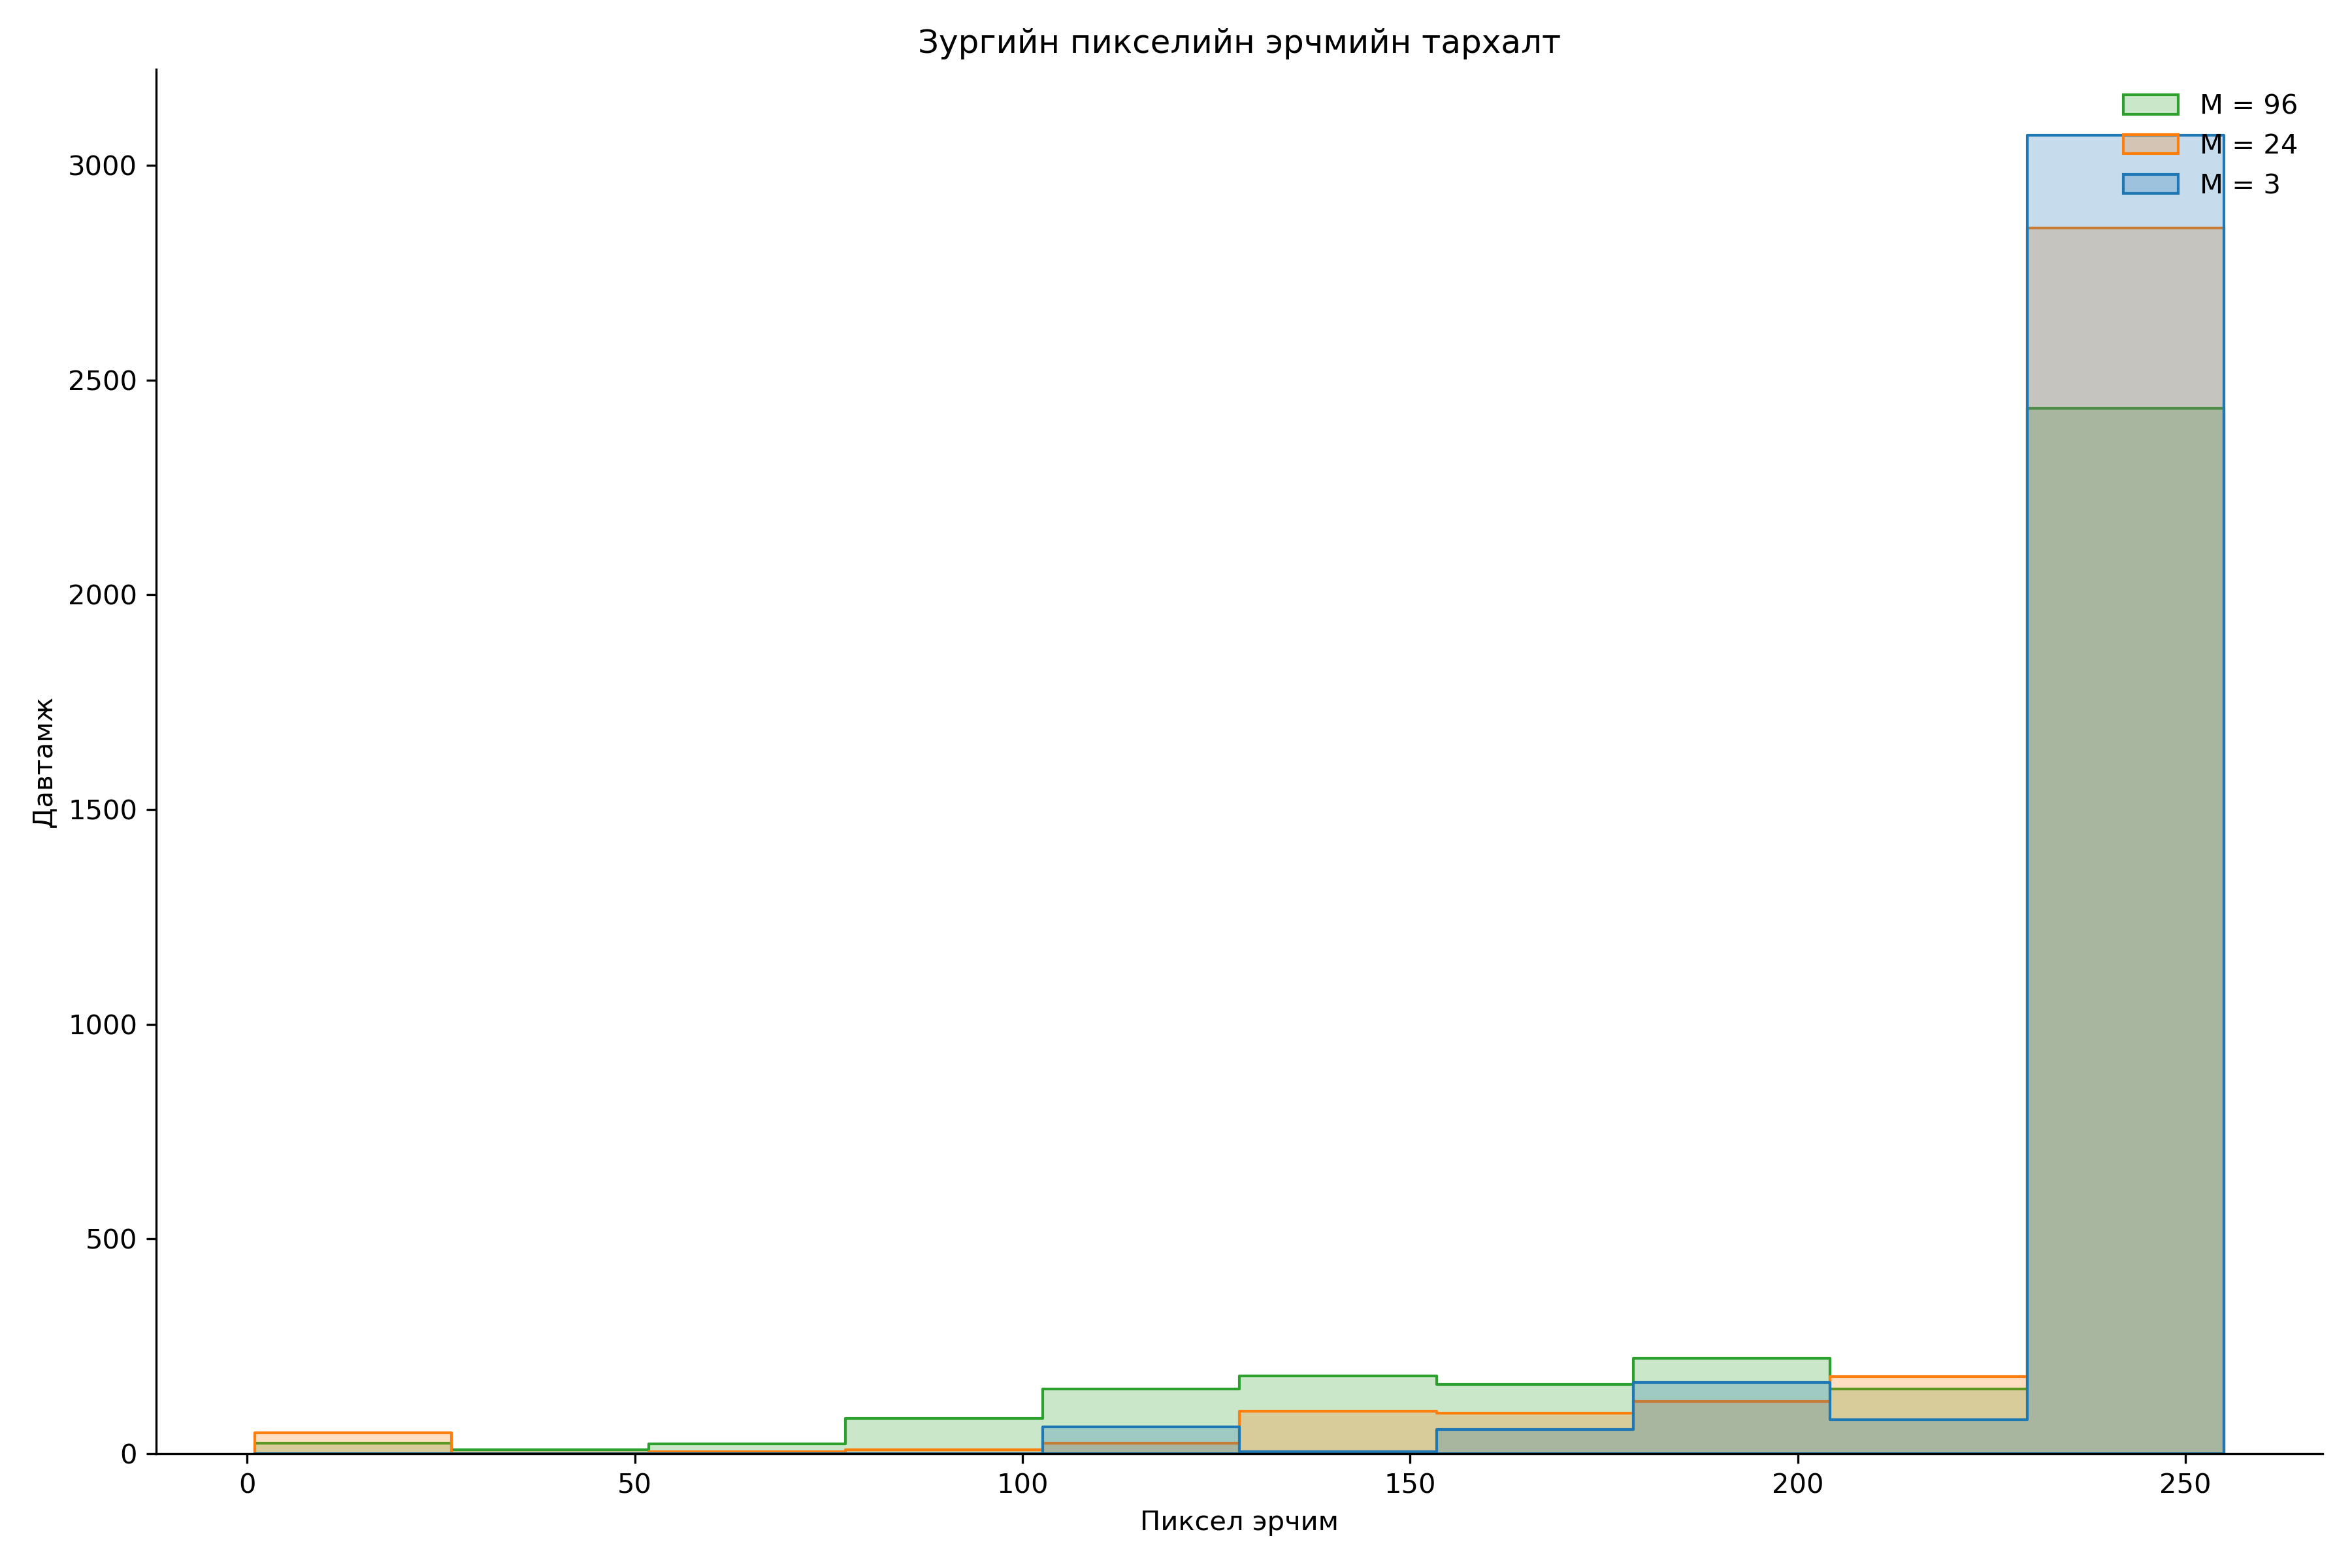
\includegraphics[scale = 0.30]{img_same_strides_diff_mask_hist.png}
  \caption[Intensity 1]{Оролтын зургийн хувьд маскийг өөрчилж шилжилтийн зайг тогтмол барьсан нь}
\end{figure}

\section{Enhancement using Arithmetic / Logic Operations}
Энд бид өгөгдсөн маскийг зурагтай үржүүлэх үйлдлүүдийг хийнэ.
\begin{figure}[H]
  \centering
  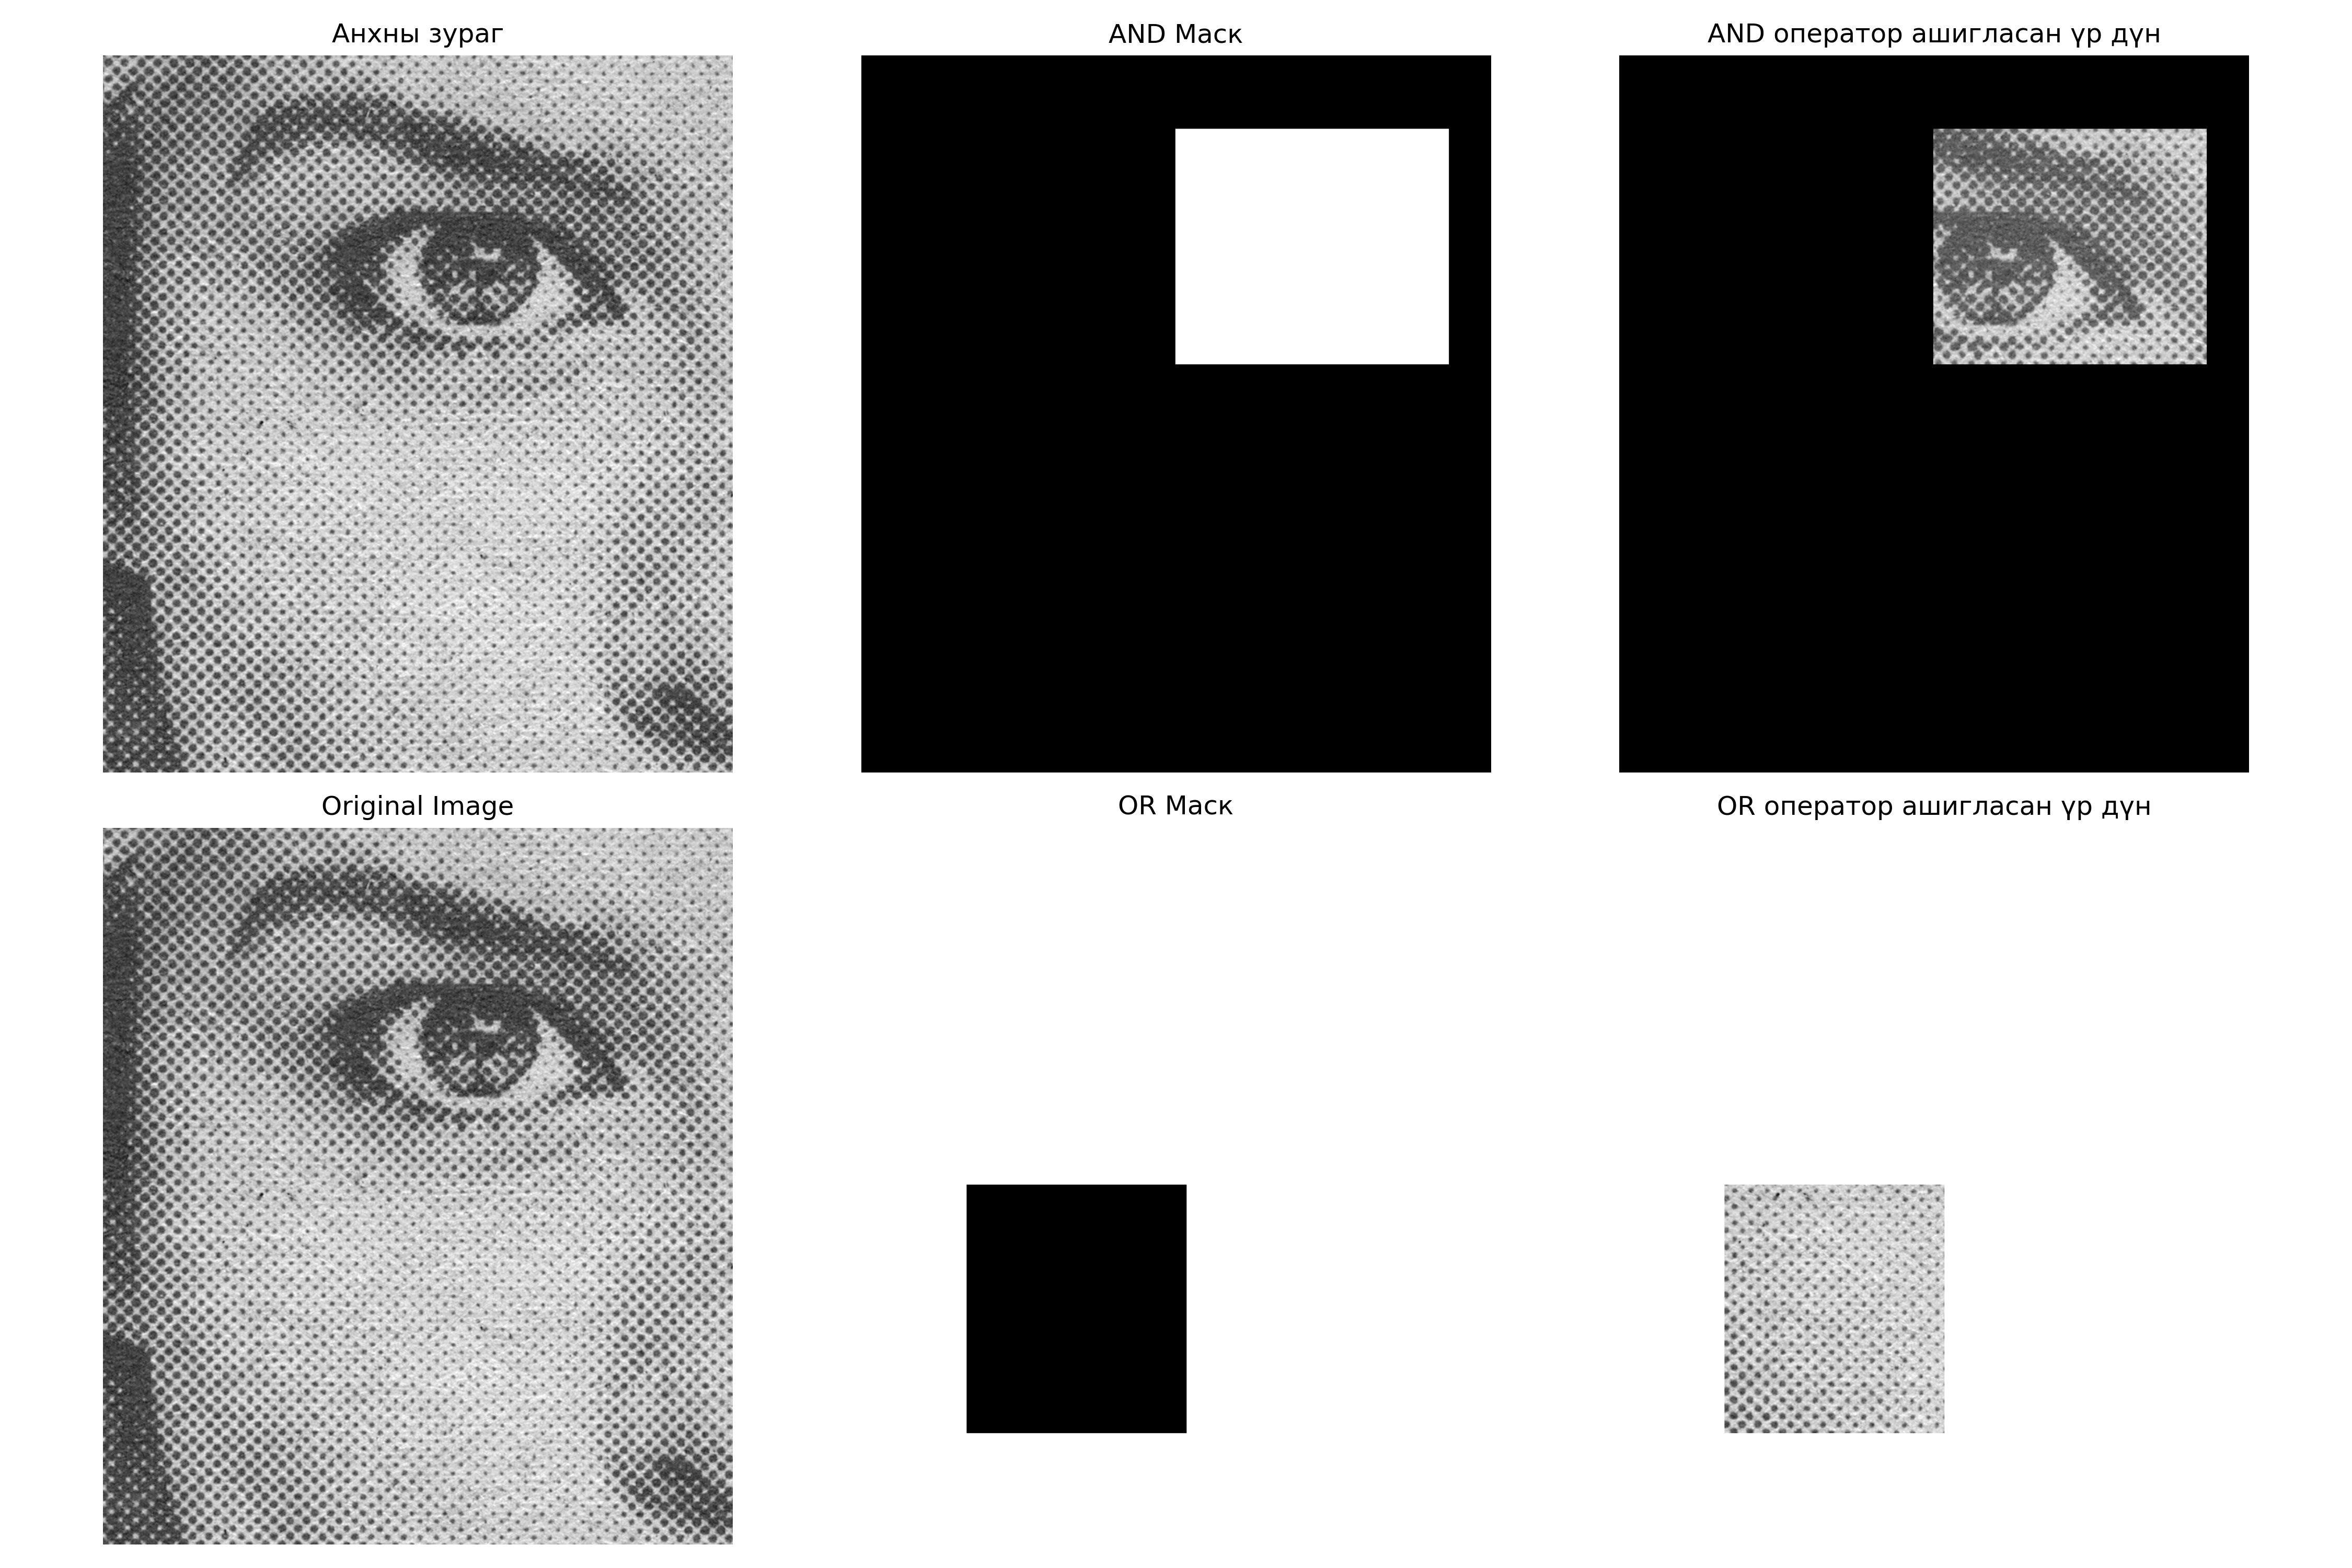
\includegraphics[scale = 0.30]{enhancement_arithmetics_1.png}
  \caption[Intensity 1]{Оролтын зураг дээрх AND болон OR масктай үржүүлсэн нь}
\end{figure}
\begin{python}
def bitwise_op(img, mask, op):
    h, w = img.shape
    img = img / 255
    res = np.zeros((h, w))
    for i in range(h):
        for j in range(w):
            if ((op == 'and') and (img[i][j] and mask[i][j])):
                res[i][j] = img[i][j]
            elif ((op == 'or') and (img[i][j] or mask[i][j])):
                if (mask[i][j] > img[i][j]):
                    res[i][j] = mask[i][j]
                else:
                    res[i][j] = img[i][j]
    return res
\end{python} \hfill \break
Дурын маск үүсгэх
\begin{python}
def transform_mask(img, mask, val):
    a = np.random.randint(img.shape[0]//2)
    b = a + np.random.randint(img.shape[0]//4, img.shape[0]//2)
    c = np.random.randint(img.shape[1]//2)
    d = c + np.random.randint(img.shape[0]//4, img.shape[1]//2)
    mask[a:b, c:d] = val

    return mask
\end{python} \hfill \break
\begin{figure}[H]
  \centering
  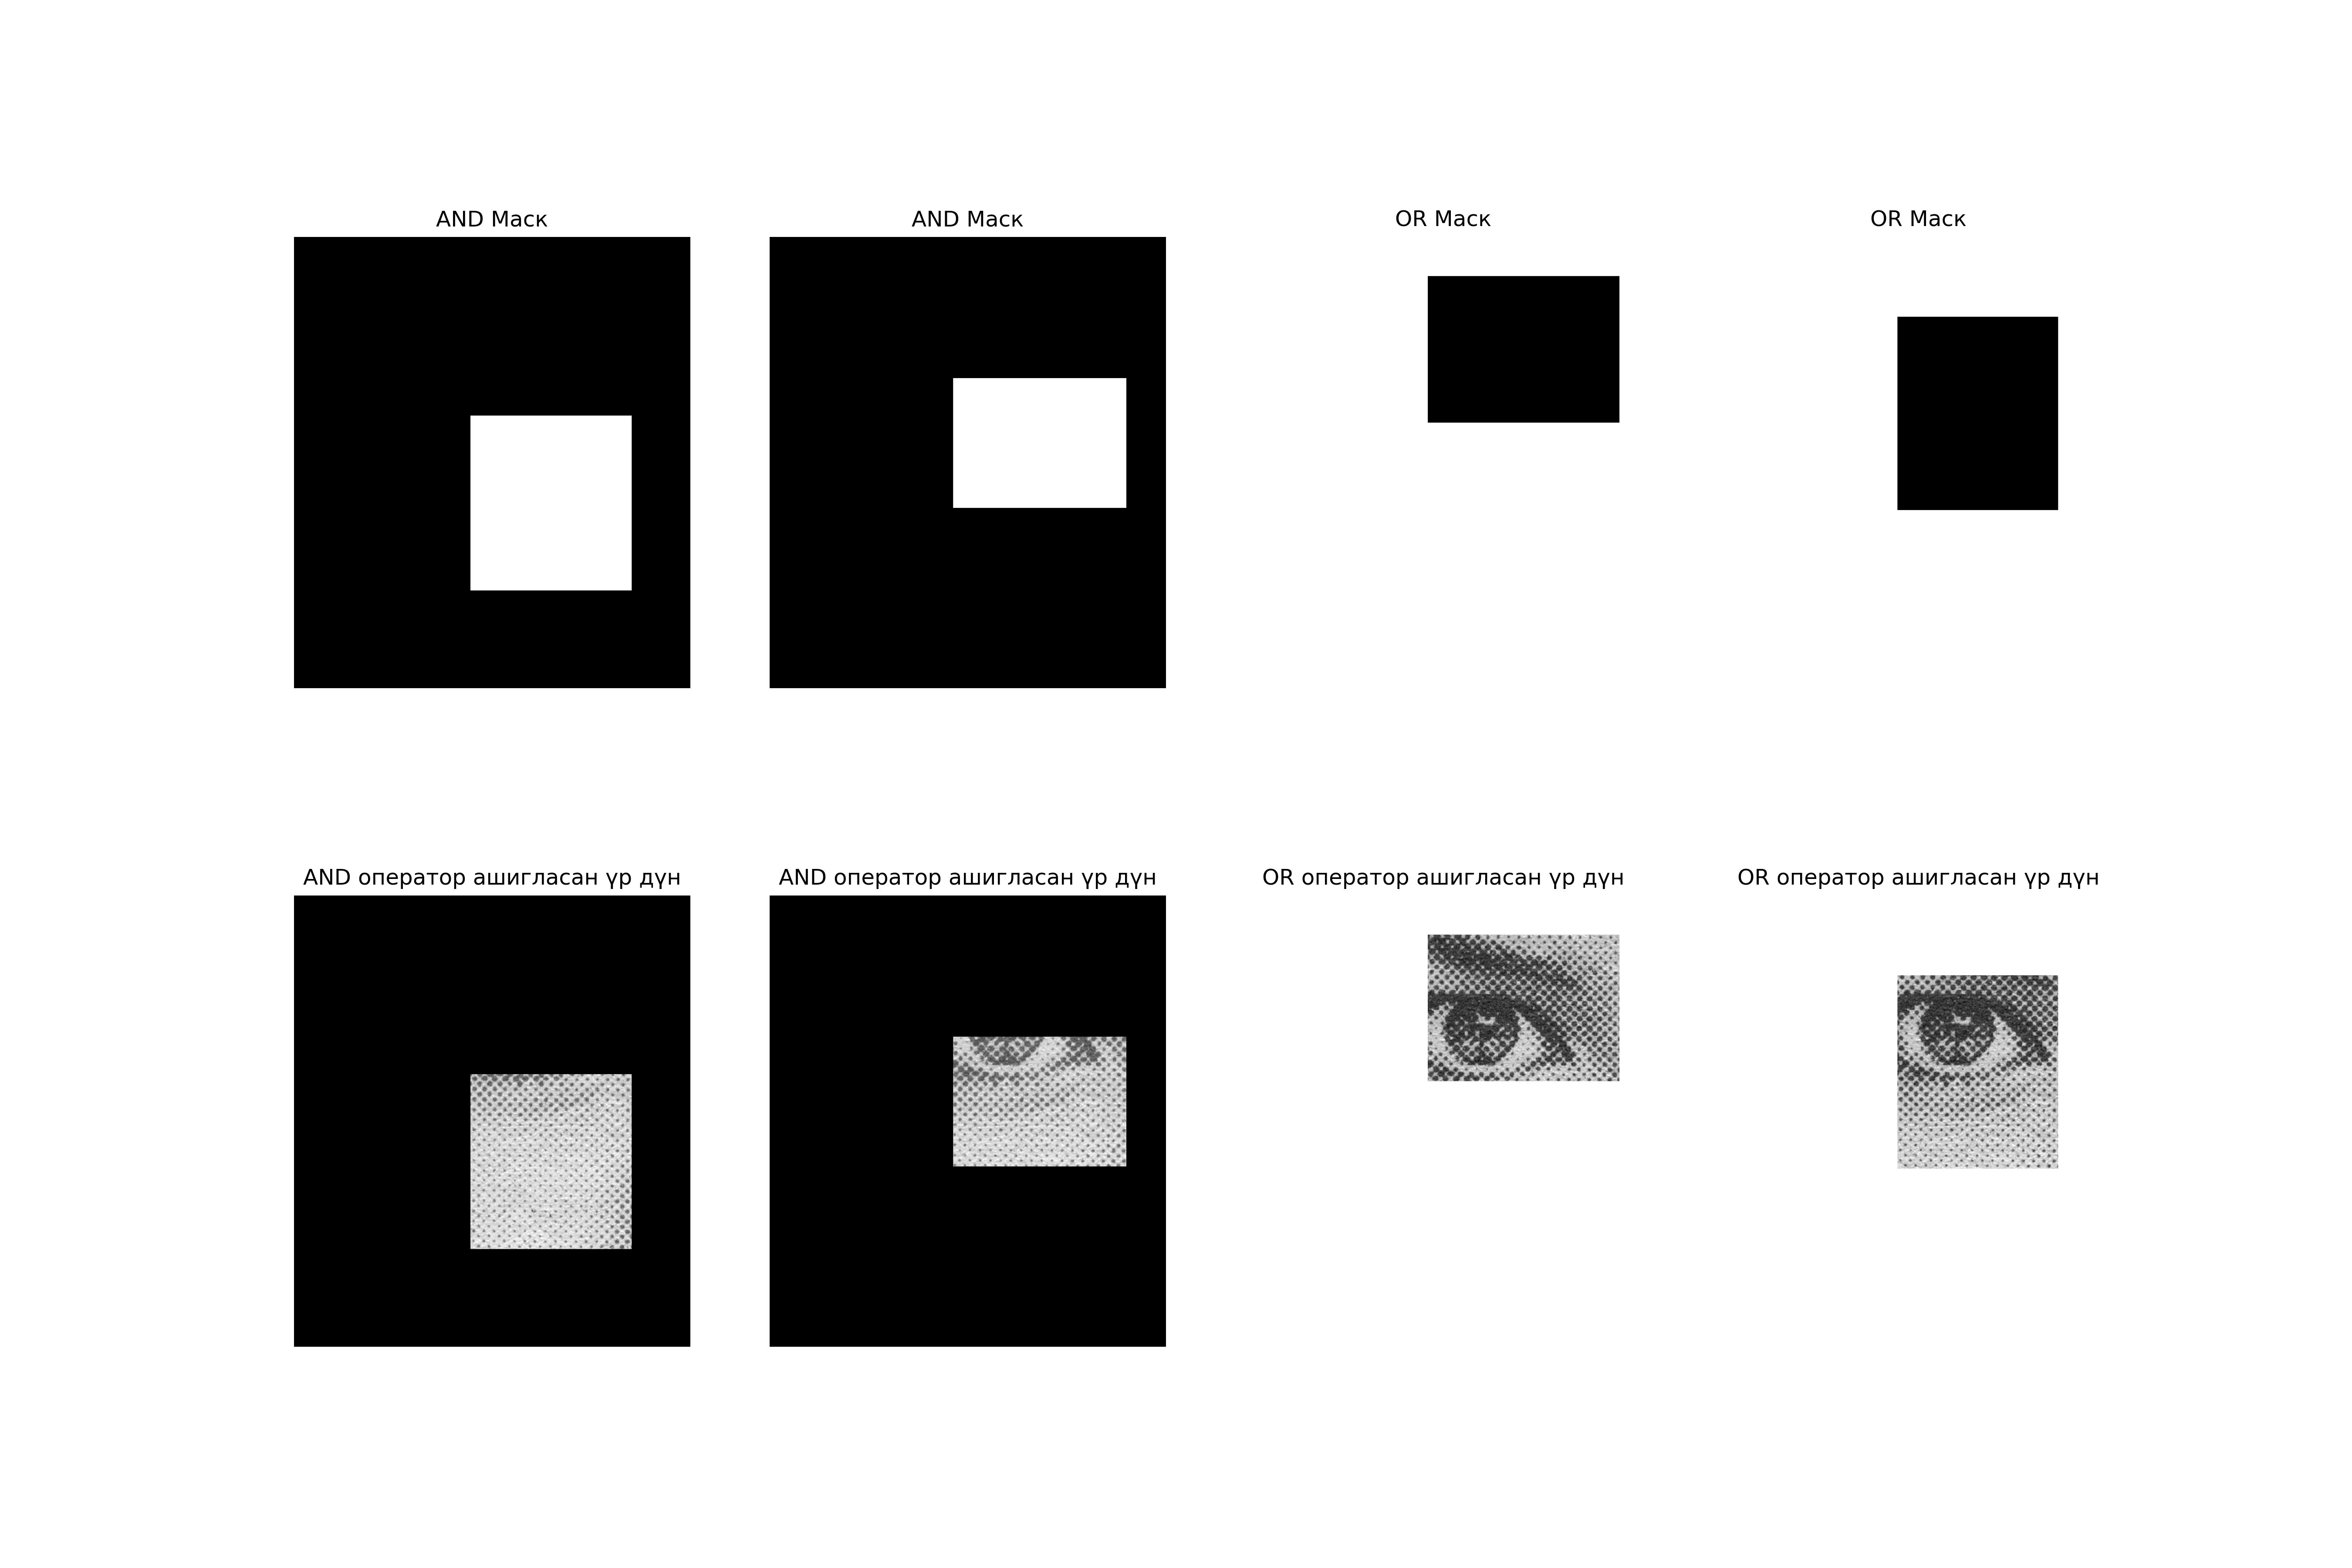
\includegraphics[scale = 0.30]{enhancement_arithmetics_2.png}
  \caption[Intensity 1]{Ялгаатай AND болон OR маск ашигласан үр дүн}
\end{figure}

\section{Smoothing Linear Filters}
Энэ хэсэгт зургийн пиксел бүрийн утгыг хөрш пикселийн утгуудын дунджаар солино \cite{gonzalez2009digital}. 
\begin{equation}
I_{3} = \frac{1}{3^2}
\begin{bmatrix}
1 & 1 & 1 \\
1 & 1 & 1 \\
1 & 1 & 1 \\
\end{bmatrix}
\end{equation}
\begin{figure}[H]
  \centering
  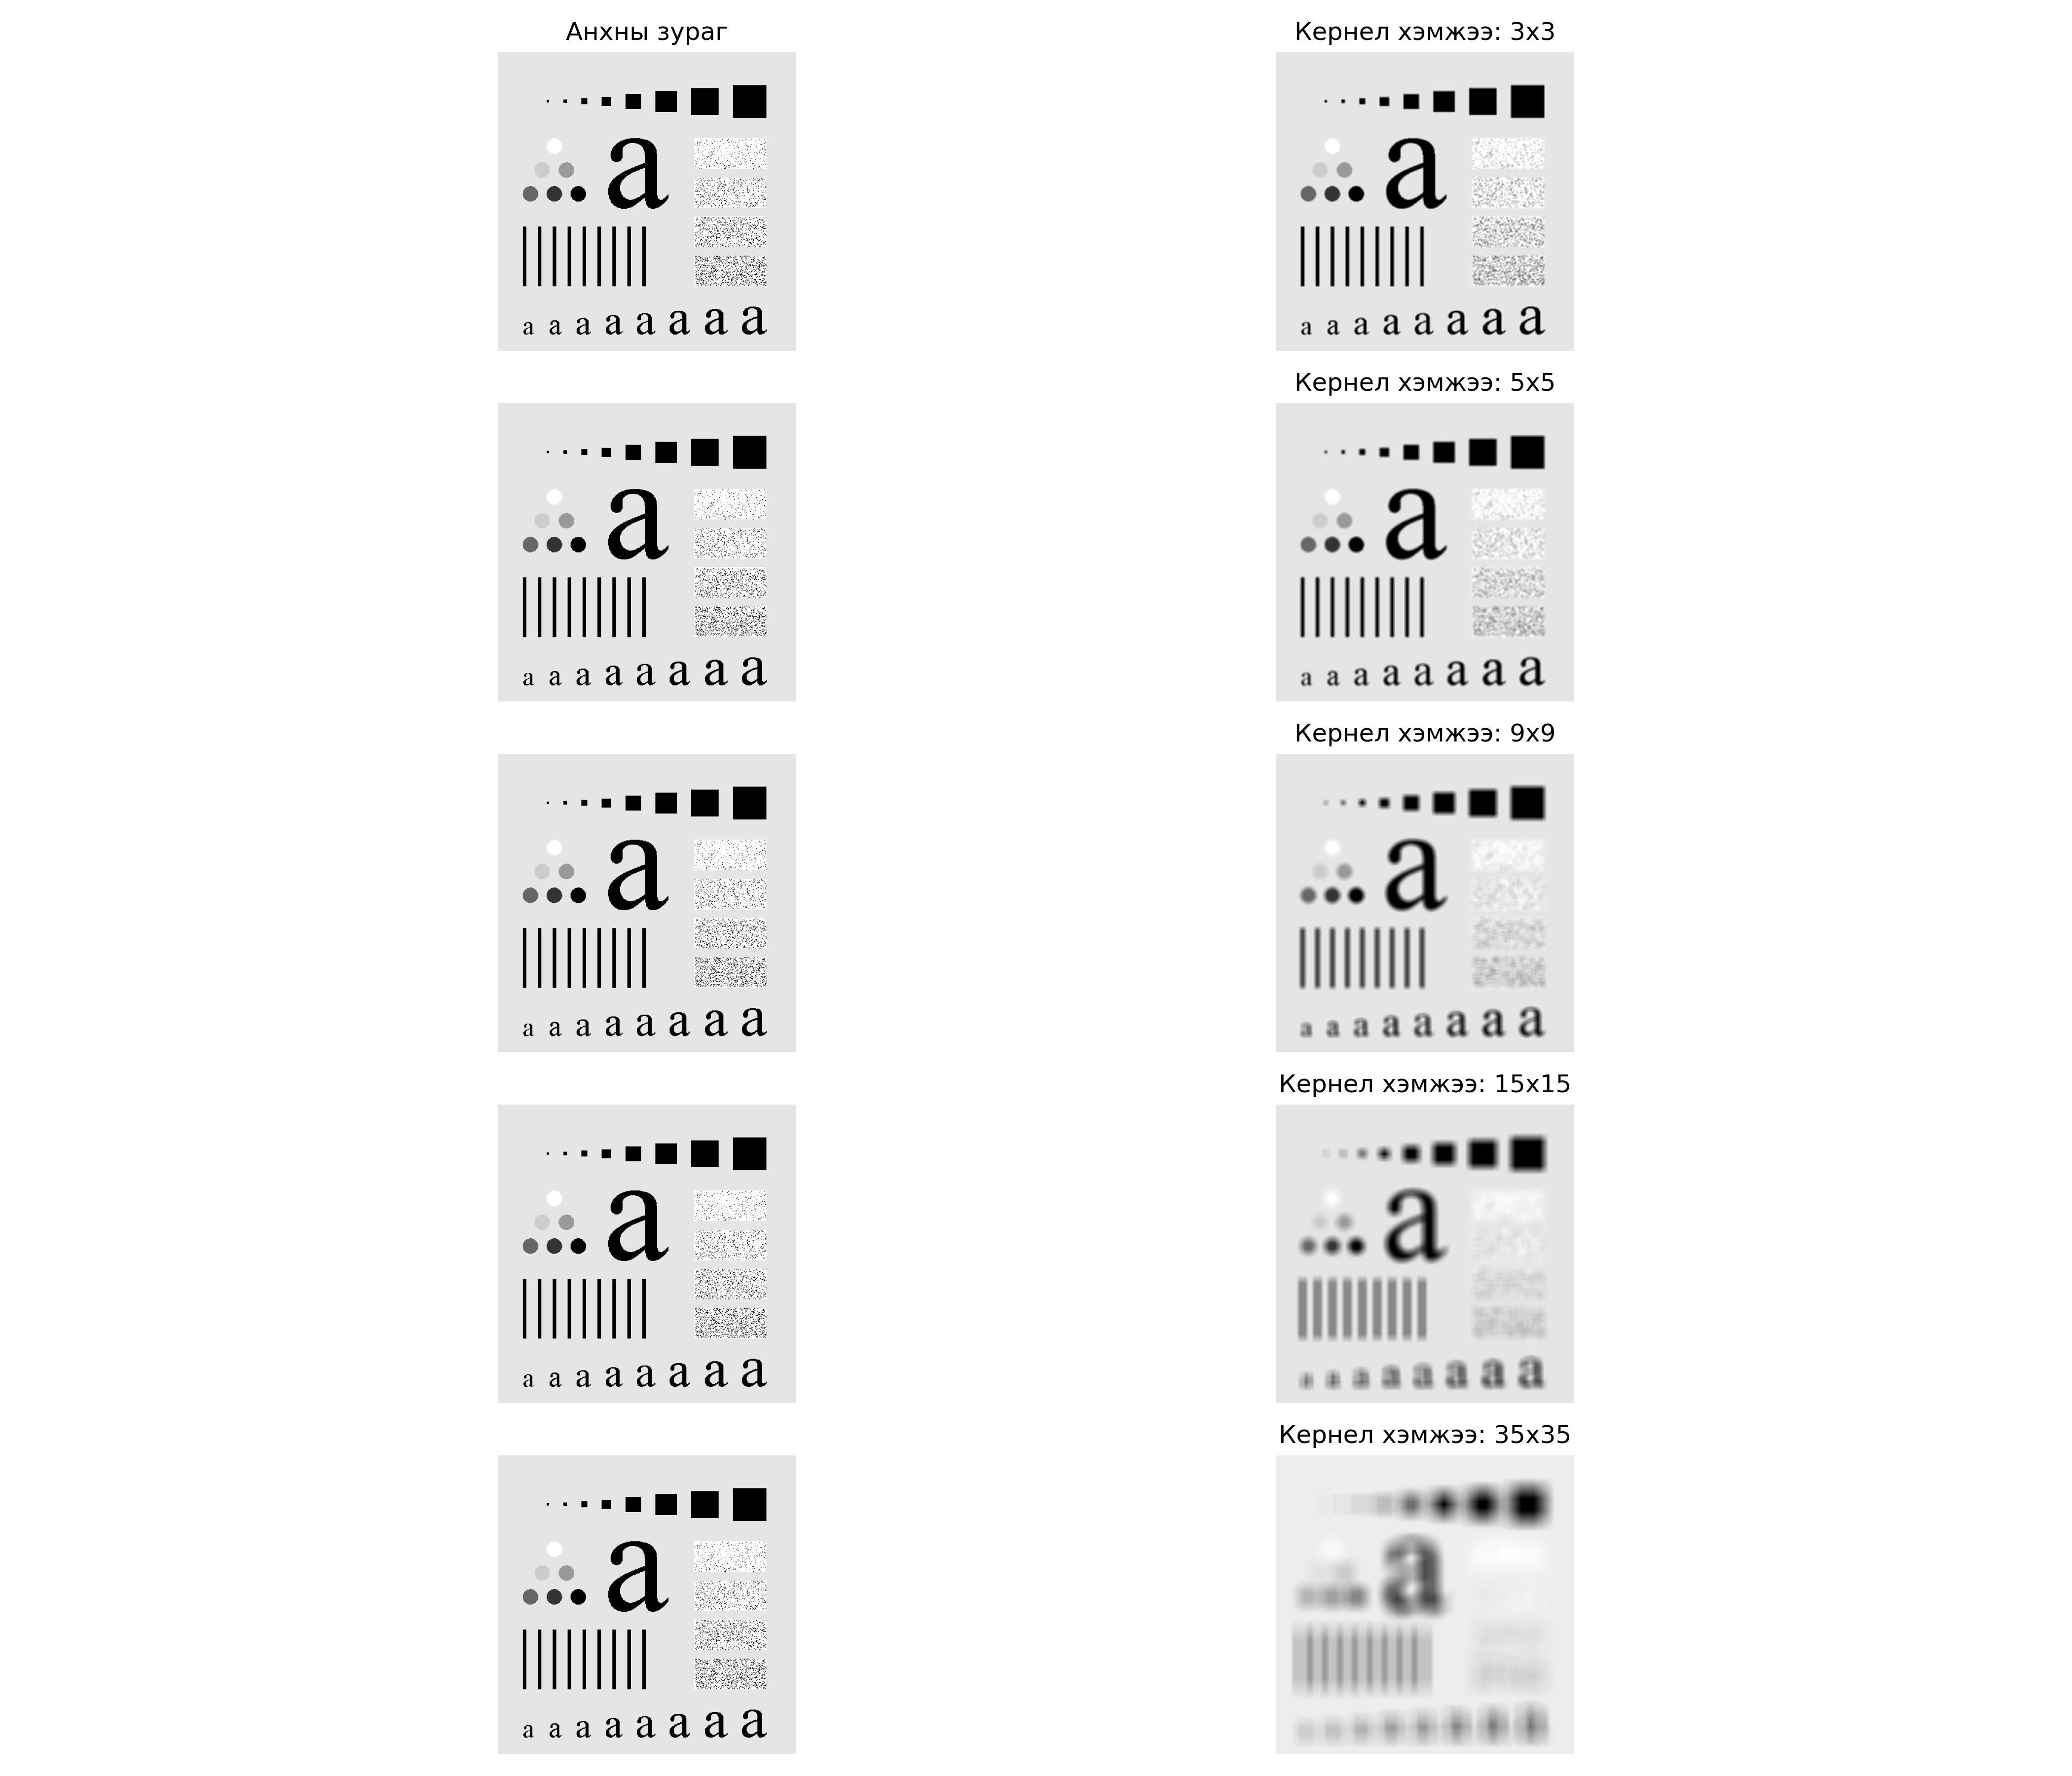
\includegraphics[scale = 0.30]{smoothing_1.png}
  \caption[Intensity 1]{Оролтын зураг болон бэлэн функц ашигласан smoothing}
\end{figure}
\begin{python}
kernel_sizes = [3, 5, 9, 15, 35]

num_rows = len(kernel_sizes)
num_cols = 2
fig, axes = plt.subplots(num_rows, num_cols, figsize = (14, 12))

for i, kernel_size in enumerate(kernel_sizes):
    kernel = np.ones((kernel_size, kernel_size), dtype = np.float32) / (kernel_size ** 2)
    smoothed_image = cv2.filter2D(img, -1, kernel)

    axes[i, 0].imshow(img, cmap = 'gray')
    if i == 0:
        axes[i, 0].set_title('Anhnii zurag')

    axes[i, 1].imshow(smoothed_image, cmap='gray')
    axes[i, 1].set_title(f'Kernel hemjee: {kernel_size}x{kernel_size}')

    axes[i, 0].axis('off')
    axes[i, 1].axis('off')


plt.tight_layout()
plt.show()
fig.savefig("./plots/smoothing_1.png", dpi = 300)
\end{python}
Харин доорх зурагт задгайгаар бичиж smoothing функц болон бэлэн функцийн үр дүнгүүдийн ялгааг харуулж байна.
\begin{figure}[H]
  \centering
  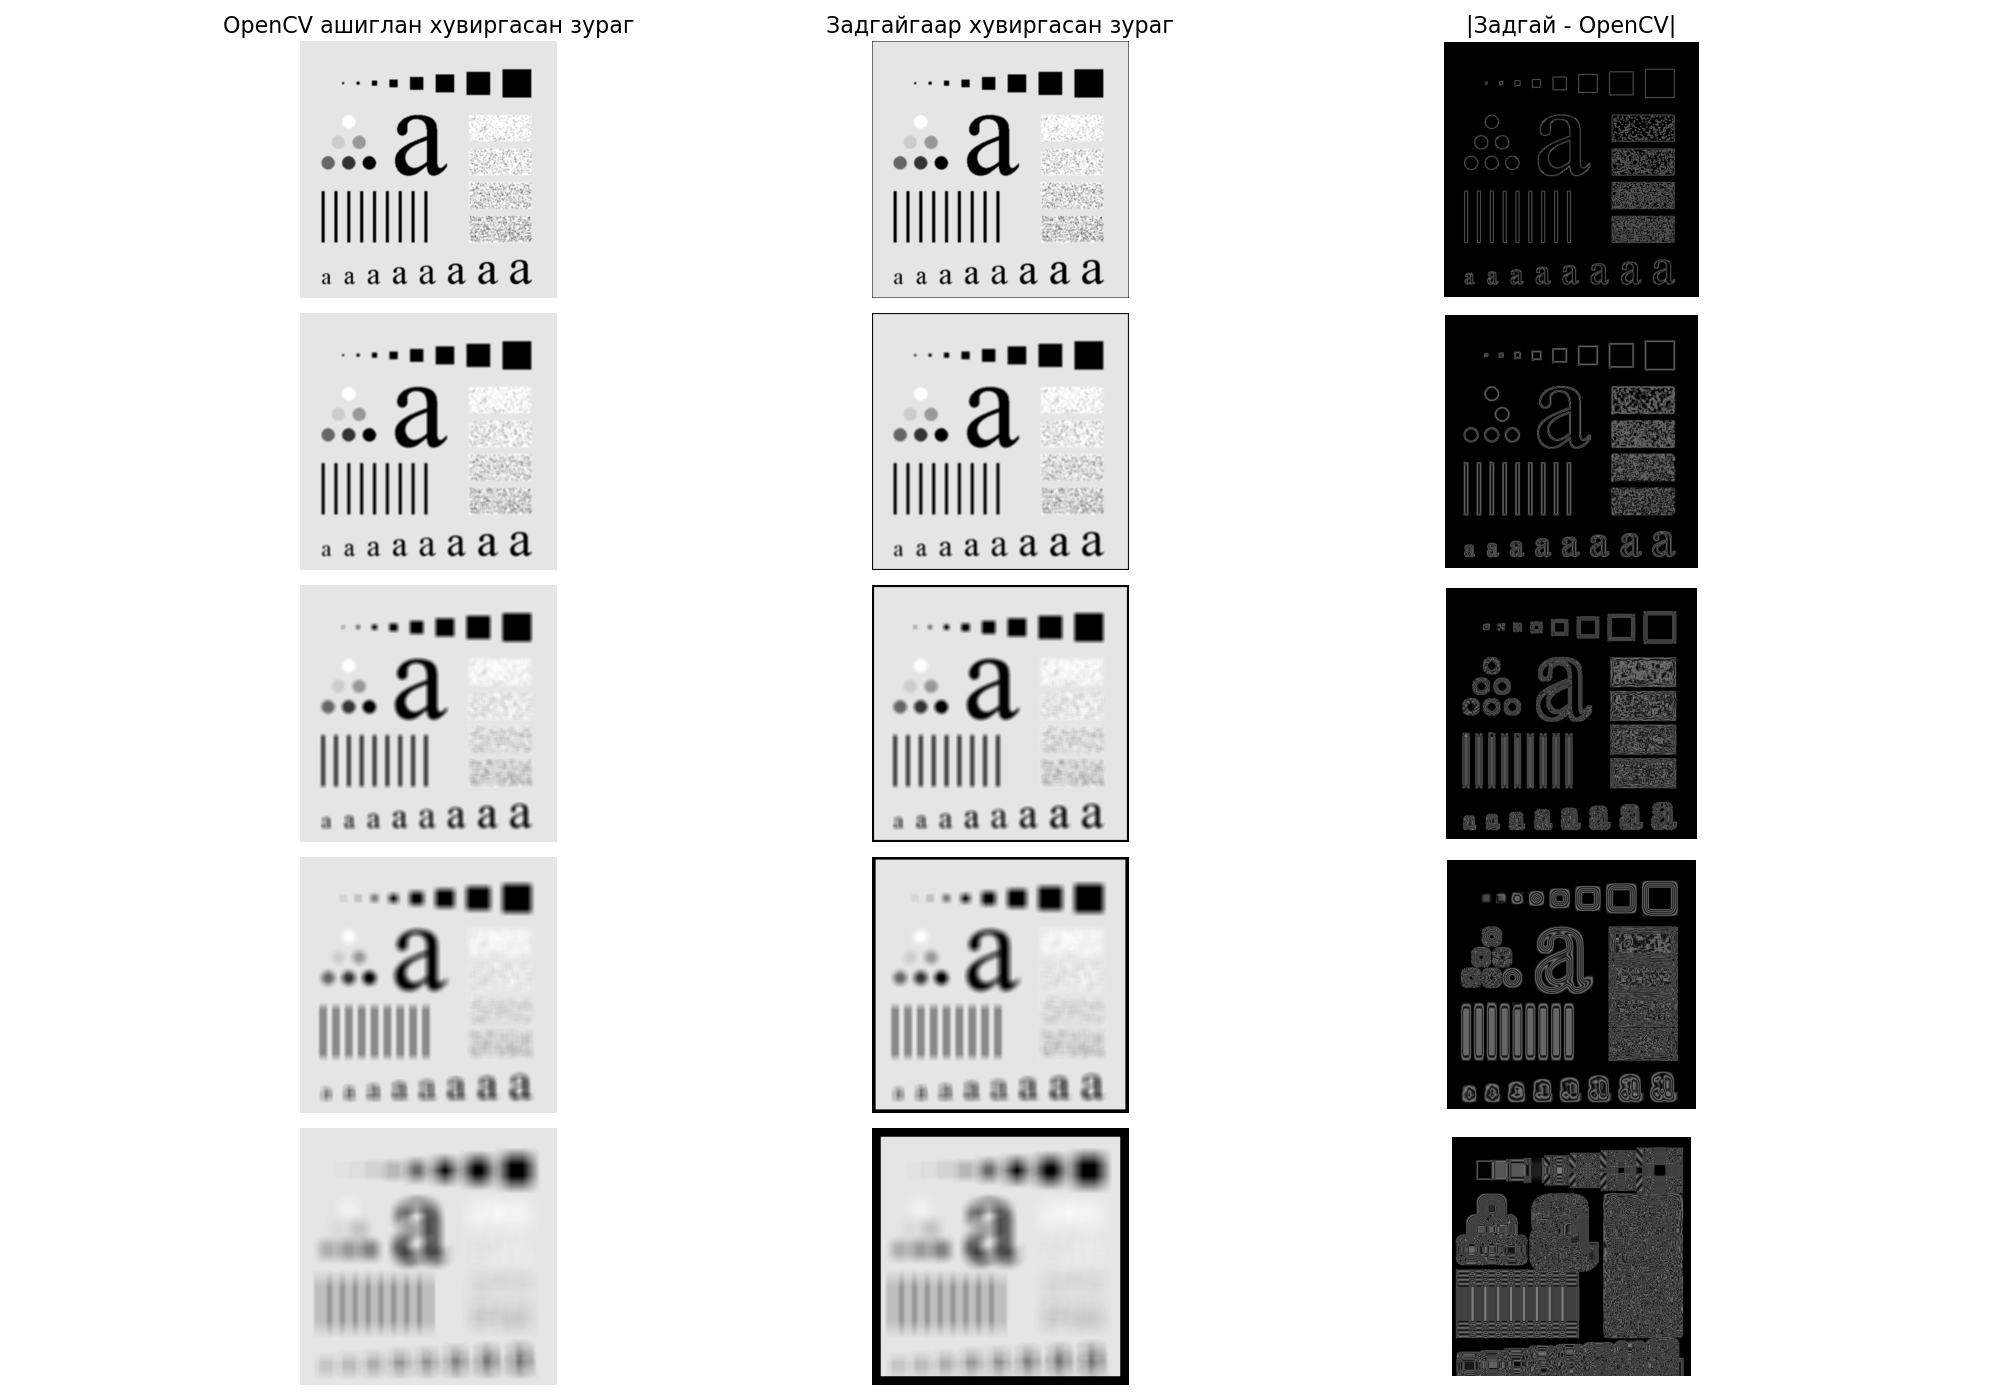
\includegraphics[scale = 0.30]{smoothing_3.png}
  \caption[Intensity 1]{Задгайгаар бичиж smoothing функц болон бэлэн функцийн үр дүнгийн ялгаа}
\end{figure}
\begin{python}
def smooth_img(img, kernel_size):
    height, width = img.shape
    kernel = np.ones((kernel_size, kernel_size), dtype = np.float32) / (kernel_size ** 2)
    smoothed_image = np.zeros((height, width), dtype = np.float32)

    kernel_iter = kernel_size // 2
    for i in range(kernel_iter, height - kernel_iter):
        for j in range(kernel_iter, width - kernel_iter):
            neighborhood = img[i - kernel_iter: i + kernel_iter + 1, j - kernel_iter: j + kernel_iter + 1]

            smoothed_pixel = np.sum(neighborhood * kernel)
            smoothed_image[i, j] = smoothed_pixel
    
    return smoothed_image
\end{python}

Одоо оролтыг зургийг өөрчилж smoothing хийе. Харин smoothing хийсний дараагаар уг зурагтаа босго тогтоож үзье.
\begin{figure}[H]
  \centering
  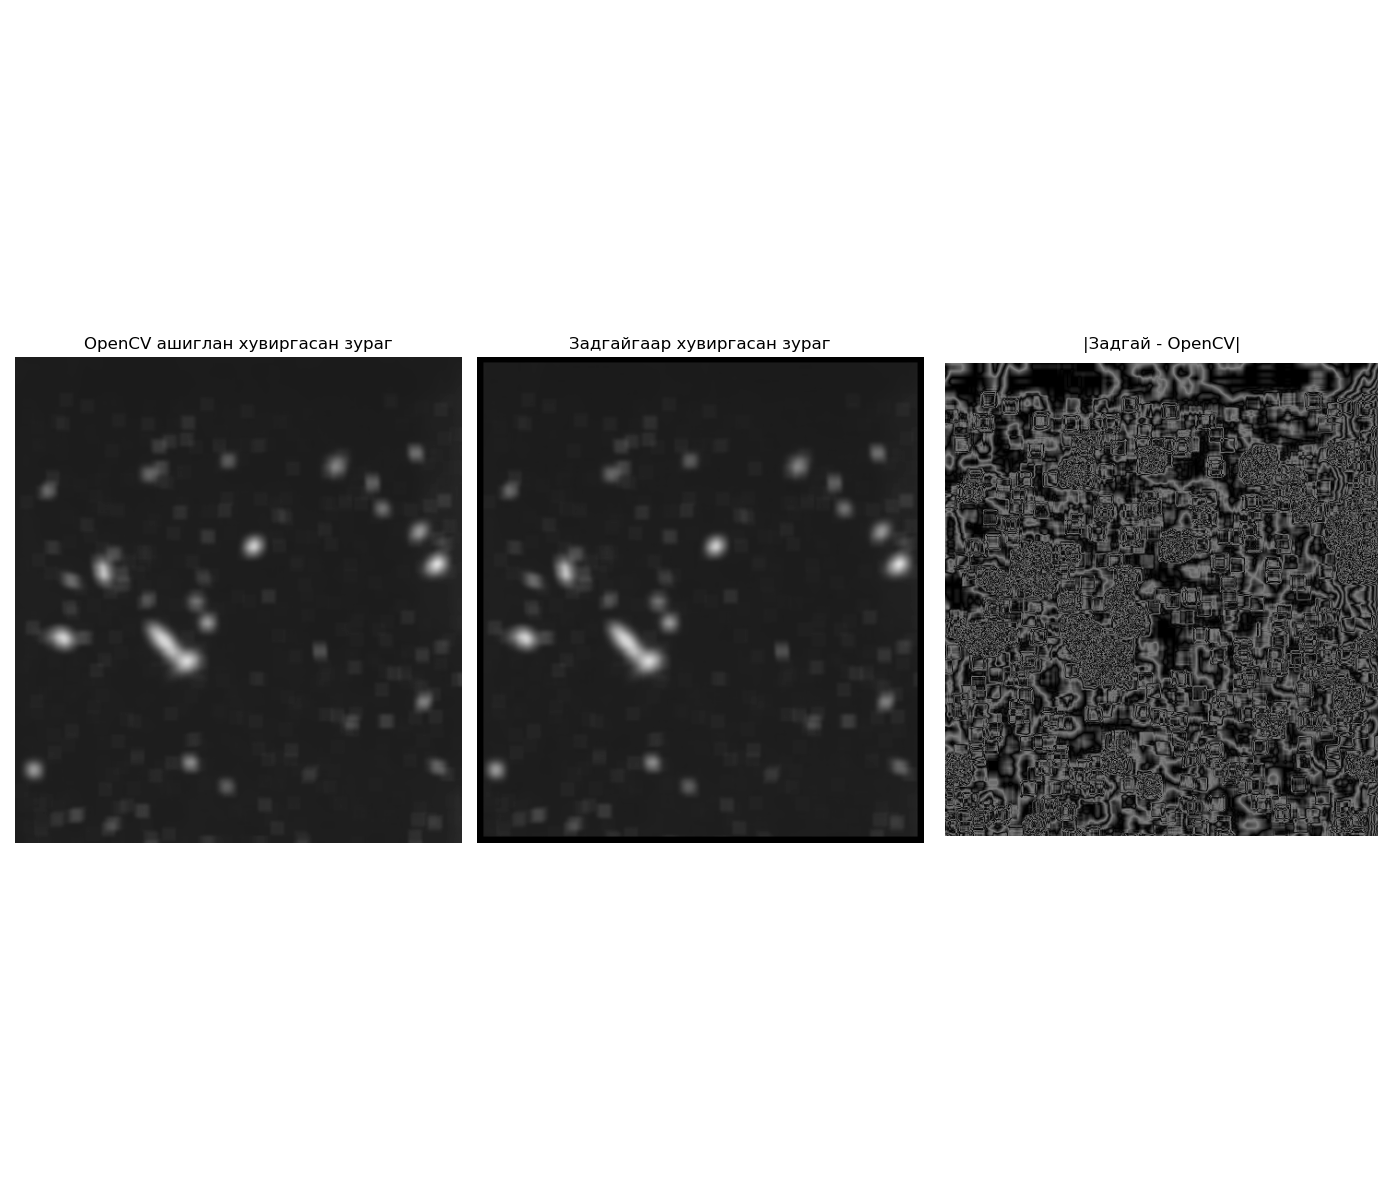
\includegraphics[scale = 0.30]{smoothing_thresh.png}
  \caption[Intensity 1]{Задгай болон бэлэн smoothing функц}
\end{figure}

Пикселийн 128 утгаар босго тогтооё.
\begin{python}
thresh = 128
smoothed_image_cv_thresh = (smoothed_image_cv > thresh)*1
smoothed_image_thresh = (smoothed_image > thresh)*1
\end{python}
\begin{figure}[H]
  \centering
  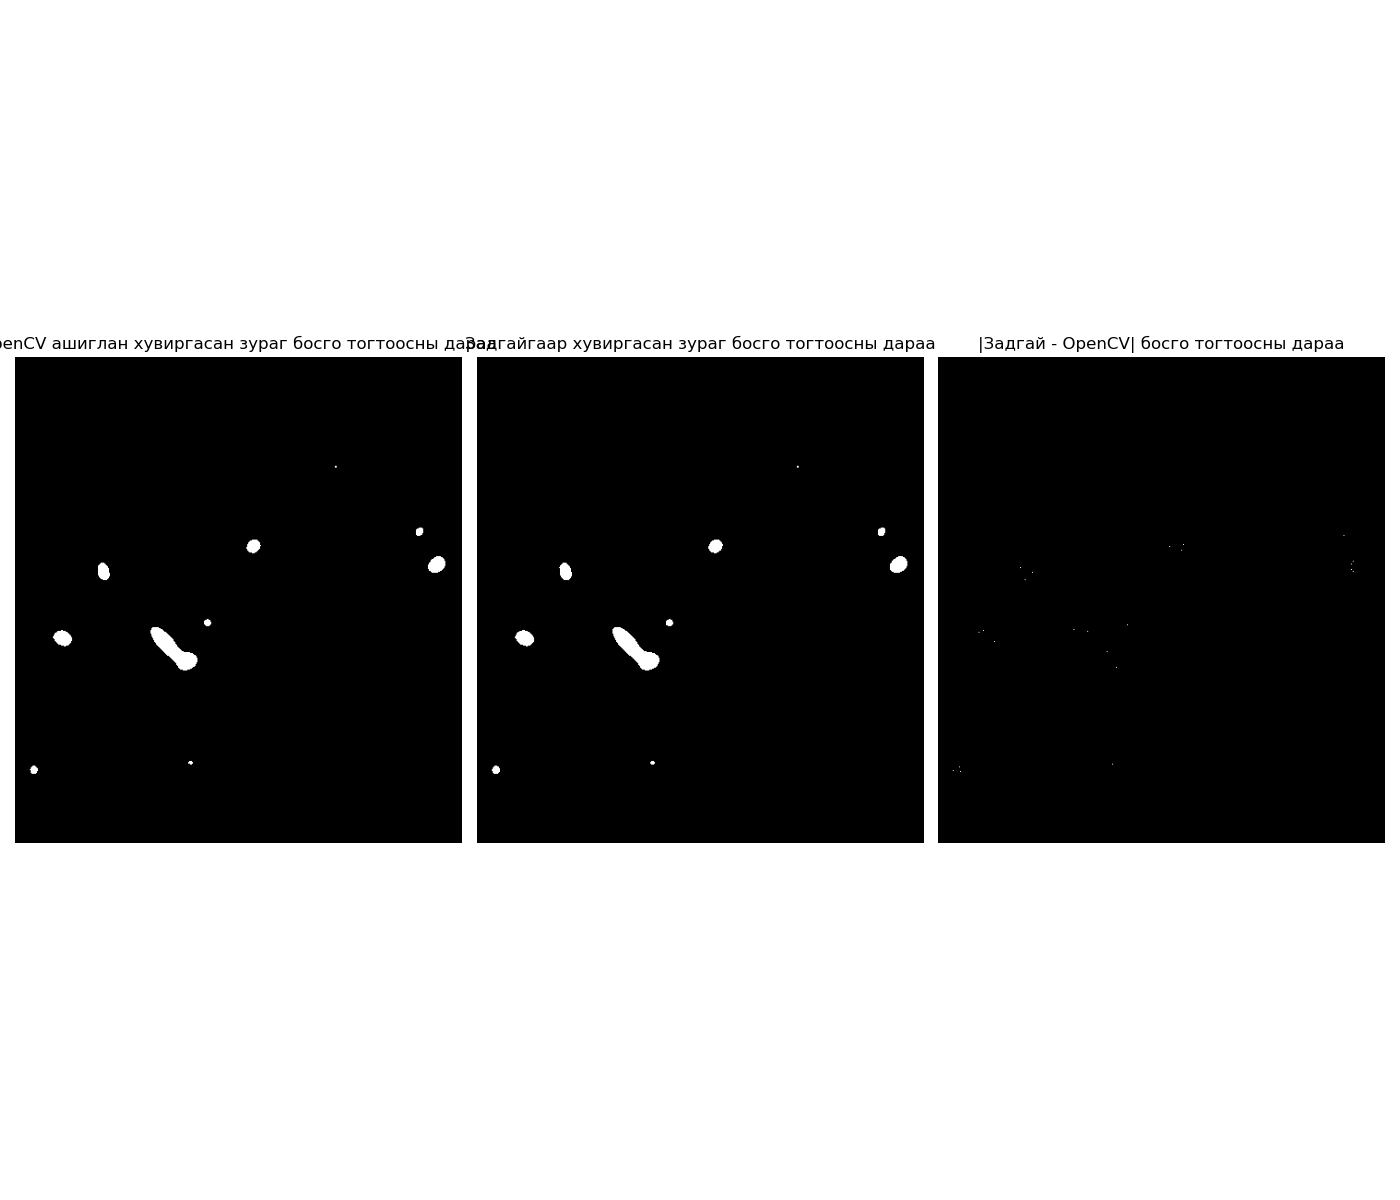
\includegraphics[scale = 0.30]{smoothing_thresh_1.png}
  \caption[Intensity 1]{Задгай болон бэлэн smoothing функцийн үр дүнд босго тогтоосон нь}
\end{figure}

\section{Дүгнэлт}
Энэ лабораторийн ажлаар зурагт боловсруулалт хийхэд шууд нэг пикселийн хувьд биш харин хэсэг бүлэг пикселийн хувьд боловсруулалт хийж сурлаа. Үүнд ялгаатай хэмжээтэй маск зургаар гүйлгэхдээ ялгаатай зайгаар гүйлгэх мөн зургийн ирмэгийн пикселүүд дээр гүйлгэхийн тулд зурагт padding нэмэх гэх мэт аргуудтай танилцлаа.
\section{Ном зүй}
\printbibliography[heading=none]
\end{document}